

\section{Detailed Data}
\label{sec:appendix}

% \setlength{\floatsep}{1mm}
% \setlength{\textfloatsep}{1mm}
% \setlength{\abovecaptionskip}{1mm}
% \setlength{\belowcaptionskip}{1mm}
% \setlength{\abovedisplayskip}{1mm}
% \setlength{\belowdisplayskip}{1mm}
% \setlength{\arraycolsep}{1mm}

\subsection{Detailed Data for \reftbl{tbl:summary-std}}

\begin{table}[htbp]
 {
 \relsize{-0.5}
 \centering
 \begin{center}
\begin{tabular}{|r|*{2}{ccc|}}
Domain & \([f,\fifo]\) & \([f,\lifo]\) & \([f,\ro]\) & \([f,h,\fifo]\) & \([f,h,\lifo]\) & \([f,h,\ro]\)\\
IPC benchmark (1104) & 443 & 558 & 448.9 \(\pm\) 1.3 & 558 & \textbf{565} & 558.9 \(\pm\) 2.1\\
airport(50) & 18 & 26 & 18 \(\pm\) 0 & \textbf{27} & 26 & 25.7 \(\pm\) 0.5\\
barman-opt11(20) & 0 & 0 & 0 \(\pm\) 0 & 0 & 0 & 0 \(\pm\) 0\\
blocks(35) & 26 & 26 & 26 \(\pm\) 0 & \textbf{28} & \textbf{28} & \textbf{28} \(\pm\) 0\\
\textbf{cybersec(19)} & 0 & 3 & 0 \(\pm\) 0 & 2 & 3 & \textbf{3.9} \(\pm\) 1.1\\
depot(22) & 5 & 5 & 5 \(\pm\) 0 & 6 & 6 & 6 \(\pm\) 0\\
driverlog(20) & 12 & 13 & 12 \(\pm\) 0 & 13 & 13 & 13 \(\pm\) 0\\
elevators-opt11(20) & 14 & 15 & 14 \(\pm\) 0 & 15 & 15 & 15 \(\pm\) 0\\
floortile-opt11(20) & 6 & 6 & 6 \(\pm\) 0 & 6 & 6 & 6 \(\pm\) 0\\
freecell(80) & 8 & 9 & 8.7 \(\pm\) 0.5 & 9 & 9 & 9 \(\pm\) 0\\
grid(5) & 1 & 1 & 1 \(\pm\) 0 & 1 & 1 & 1 \(\pm\) 0\\
gripper(20) & 6 & 6 & 6 \(\pm\) 0 & 6 & 6 & 6 \(\pm\) 0\\
hanoi(30) & 12 & 12 & 12 \(\pm\) 0 & 12 & 12 & 12 \(\pm\) 0\\
logistics00(28) & 16 & 18 & 16 \(\pm\) 0 & \textbf{20} & \textbf{20} & \textbf{20} \(\pm\) 0\\
miconic(150) & 68 & 140 & 68 \(\pm\) 0 & 140 & 140 & 140 \(\pm\) 0\\
mprime(35) & 20 & \textbf{22} & 19.9 \(\pm\) 0.3 & 21 & 21 & 20.9 \(\pm\) 0.3\\
mystery(30) & 15 & 16 & 15 \(\pm\) 0 & 16 & 16 & 15.2 \(\pm\) 0.4\\
nomystery-opt11(20) & 12 & 13 & 12 \(\pm\) 0 & \textbf{14} & \textbf{14} & \textbf{14} \(\pm\) 0\\
\textbf{openstacks-opt11(20)} & 11 & \textbf{18} & 11.2 \(\pm\) 0.4 & 11 & \textbf{18} & 11.7 \(\pm\) 0.5\\
parcprinter-opt11(20) & 12 & 13 & 12 \(\pm\) 0 & 13 & 13 & 13 \(\pm\) 0\\
parking-opt11(20) & 1 & 1 & 1 \(\pm\) 0 & 1 & 1 & 1 \(\pm\) 0\\
pathways(30) & 4 & 5 & 4 \(\pm\) 0 & 5 & 5 & 5 \(\pm\) 0\\
pegsol-opt11(20) & 17 & 17 & 17 \(\pm\) 0 & 17 & 17 & 17 \(\pm\) 0\\
pipesworld-notankage(50) & 13 & 13 & 13 \(\pm\) 0 & 14 & 14 & 14.6 \(\pm\) 0.5\\
pipesworld-tankage(50) & 7 & 8 & 8 \(\pm\) 0 & 8 & 8 & 8 \(\pm\) 0\\
psr-small(50) & 48 & 48 & 48 \(\pm\) 0 & 48 & 48 & 48 \(\pm\) 0\\
rovers(40) & 7 & 7 & 7 \(\pm\) 0 & 7 & 7 & 7 \(\pm\) 0\\
scanalyzer-opt11(20) & 4 & \textbf{10} & 5.4 \(\pm\) 0.7 & \textbf{10} & \textbf{10} & \textbf{10} \(\pm\) 0\\
sokoban-opt11(20) & 19 & 19 & 19 \(\pm\) 0 & 19 & 19 & 19 \(\pm\) 0\\
storage(30) & 14 & 14 & 14 \(\pm\) 0 & 14 & 14 & 14 \(\pm\) 0\\
tidybot-opt11(20) & 11 & 12 & 11 \(\pm\) 0 & 12 & 12 & 12 \(\pm\) 0\\
tpp(30) & 6 & 6 & 6 \(\pm\) 0 & 6 & 6 & 6 \(\pm\) 0\\
transport-opt11(20) & 6 & 6 & 6 \(\pm\) 0 & 6 & 6 & 6 \(\pm\) 0\\
visitall-opt11(20) & 9 & 10 & 9.4 \(\pm\) 0.5 & 10 & 10 & 10 \(\pm\) 0\\
woodworking-opt11(20) & 6 & 9 & 8.2 \(\pm\) 0.4 & \textbf{10} & \textbf{10} & \textbf{10} \(\pm\) 0\\
zenotravel(20) & 9 & \textbf{11} & 9 \(\pm\) 0 & \textbf{11} & \textbf{11} & \textbf{11} \(\pm\) 0\\
\end{tabular}
\end{center}

 \caption{
 Coverage comparison (the number of instances solved in 5min, 4GB, LMcut
 heuristics) among
 the standard baseline tie-breaking algorithms. We highlight the
 best results when the difference between the maximum and the minimum coverage exceeds 2.
 }
 \label{tbl:lmcut-ipc-std}
 }
\end{table}

\begin{table}[htbp]
 {
 \relsize{-0.5}
 \centering
 \begin{center}
\begin{tabular}{|r|*{2}{ccc|}}
Domain & $[f,\fifo]$ & $[f,\lifo]$ & $[f,\ro]$ & $[f,h,\fifo]$ & $[f,h,\lifo]$ & $[f,h,\ro]$\\
IPC benchmark (1104) & 460 & 490 & 460.9 $\pm$ 1.6 & 491 & \textbf{496} & 489.4 $\pm$ 1.0\\
airport(50) & 9 & 9 & 9 $\pm$ 0 & 9 & 9 & 9 $\pm$ 0\\
barman-opt11(20) & 4 & 4 & 4 $\pm$ 0 & 4 & 4 & 4 $\pm$ 0\\
blocks(35) & 21 & 22 & 21 $\pm$ 0 & 22 & 22 & 22 $\pm$ 0\\
\textbf{cybersec(19)} & 0 & 0 & 0 $\pm$ 0 & 0 & 0 & 0 $\pm$ 0\\
depot(22) & 5 & 6 & 5 $\pm$ 0 & 6 & 6 & 5 $\pm$ 0\\
driverlog(20) & 12 & 12 & 12 $\pm$ 0 & 12 & 12 & 12 $\pm$ 0\\
elevators-opt11(20) & 13 & 13 & 13 $\pm$ 0 & 13 & 13 & 13 $\pm$ 0\\
floortile-opt11(20) & 5 & 6 & 5 $\pm$ 0 & 6 & 6 & 6 $\pm$ 0\\
freecell(80) & 15 & 16 & 15 $\pm$ 0 & \textbf{17} & \textbf{17} & 16 $\pm$ 0\\
grid(5) & 2 & 2 & 2 $\pm$ 0 & 2 & 2 & 2 $\pm$ 0\\
gripper(20) & 8 & \textbf{20} & 8 $\pm$ 0 & \textbf{20} & \textbf{20} & \textbf{20} $\pm$ 0\\
hanoi(30) & 14 & 14 & 14 $\pm$ 0 & 14 & 14 & 14 $\pm$ 0\\
logistics00(28) & 20 & 20 & 20 $\pm$ 0 & 20 & 20 & 20 $\pm$ 0\\
miconic(150) & 68 & \textbf{73} & 68.3 $\pm$ 0.7 & \textbf{73} & \textbf{73} & \textbf{73.2} $\pm$ 0.4\\
mprime(35) & 23 & 23 & 22 $\pm$ 0 & 23 & \textbf{24} & 23.7 $\pm$ 0.5\\
mystery(30) & 15 & 15 & 15 $\pm$ 0 & 15 & 16 & 15 $\pm$ 0\\
nomystery-opt11(20) & 17 & 18 & 17.8 $\pm$ 0.4 & 18 & 18 & 18 $\pm$ 0\\
\textbf{openstacks-opt11(20)} & 15 & \textbf{19} & 15.4 $\pm$ 0.5 & 15 & \textbf{19} & 15.4 $\pm$ 0.5\\
parcprinter-opt11(20) & 10 & 10 & 10 $\pm$ 0 & 10 & 10 & 10 $\pm$ 0\\
parking-opt11(20) & 1 & 1 & 1 $\pm$ 0 & 1 & 1 & 1 $\pm$ 0\\
pathways(30) & 4 & 4 & 4 $\pm$ 0 & 4 & 4 & 4 $\pm$ 0\\
pegsol-opt11(20) & 17 & \textbf{19} & 17.2 $\pm$ 0.4 & \textbf{19} & \textbf{19} & \textbf{19} $\pm$ 0\\
pipesworld-notankage(50) & 9 & 9 & 8.9 $\pm$ 0.3 & 10 & 10 & 9.9 $\pm$ 0.3\\
pipesworld-tankage(50) & 13 & 13 & 13.1 $\pm$ 0.3 & 13 & 13 & 13.2 $\pm$ 0.4\\
psr-small(50) & 50 & 50 & 50 $\pm$ 0 & 50 & 50 & 50 $\pm$ 0\\
rovers(40) & 6 & \textbf{8} & 6.1 $\pm$ 0.3 & \textbf{8} & \textbf{8} & \textbf{8} $\pm$ 0\\
scanalyzer-opt11(20) & 10 & 10 & 10 $\pm$ 0 & 10 & 10 & 10 $\pm$ 0\\
sokoban-opt11(20) & 20 & 20 & 20 $\pm$ 0 & 20 & 20 & 20 $\pm$ 0\\
storage(30) & 15 & 15 & 15 $\pm$ 0 & 15 & 15 & 15 $\pm$ 0\\
tidybot-opt11(20) & 0 & 0 & 0 $\pm$ 0 & 0 & 0 & 0 $\pm$ 0\\
tpp(30) & 6 & 6 & 6 $\pm$ 0 & 7 & 6 & 6 $\pm$ 0\\
transport-opt11(20) & 7 & 7 & 7 $\pm$ 0 & 7 & 7 & 7 $\pm$ 0\\
visitall-opt11(20) & 9 & 9 & 9 $\pm$ 0 & 9 & 9 & 9 $\pm$ 0\\
woodworking-opt11(20) & 7 & 7 & 7 $\pm$ 0 & 7 & 7 & 7 $\pm$ 0\\
zenotravel(20) & 10 & 10 & 10 $\pm$ 0 & \textbf{12} & \textbf{12} & \textbf{12} $\pm$ 0\\
\end{tabular}
\end{center}

 \caption{
 Coverage comparison (the number of instances solved in 5min, 4GB, M\&S heuristics) among
 the standard baseline tie-breaking algorithms. We highlight the
 best results when the difference between the maximum and the minimum coverage exceeds 2.
 }
 \label{tbl:mands-ipc-std}
 }
\end{table}

% % This comparison can be removed even from the appendix.
% % The result is not essential. Furthermore,
% % these numbers can be extracted from the other tables.
%
% \clearpage
% \subsection{\mands Data for \reftbl{tbl:lmcut-zerocost-std}}
% 
% \begin{table}[htbp]
%  \centering
%  \begin{center}
\begin{tabular}{|lc|cr|}
 & \([f,h,\fifo]\) & \([f,h,\fifo]\) & \\
depot(22) & 6 & 5 & depot-fuel(22)\\
driverlog(20) & 12 & 9 & driverlog-fuel(20)\\
elevators-opt11(20) & 13 & 8 & elevators-up(20)\\
floortile-opt11(20) & 6 & 8 & floortile-ink(20)\\
grid(5) & 2 & 2 & grid-fuel(5)\\
gripper(20) & 20 & 20 & gripper-move(20)\\
logistics00(28) & 20 & 16 & logistics00-fuel(28)\\
mprime(35) & 23 & 21 & mprime-succumb(35)\\
nomystery-opt11(20) & 18 & 16 & nomystery-fuel(20)\\
parking-opt11(20) & 1 & 0 & parking-movecc(20)\\
pathways(30) & 4 & 4 & pathways-fuel(30)\\
rovers(40) & 8 & 8 & rovers-fuel(40)\\
scanalyzer-opt11(20) & 10 & 11 & scanalyzer-analyze(20)\\
sokoban-opt11(20) & 20 & 19 & sokoban-pushgoal(20)\\
storage(30) & 15 & 4 & storage-lift(20)\\
tidybot-opt11(20) & 0 & 0 & tidybot-motion(20)\\
tpp(30) & 7 & 9 & tpp-fuel(30)\\
woodworking-opt11(20) & 7 & 7 & woodworking-cut(20)\\
zenotravel(20) & 12 & 10 & zenotravel-fuel(20)\\
\end{tabular}
\end{center}

%  \caption{
%  Coverage comparison (the number of instances solved) 
%  between the original IPC instances and the modified Zerocost instances,
%  using the same configuration and experimental setting (5min, 4GB, \mands heuristics).
%  This table does not include domains where the total number of instances
%  differ in the Zerocost domain and the original IPC domain. The results in
%  those domains are available in the later sections.
%  }
%  \label{tbl:mands-zerocost-std}
% \end{table}

\clearpage
\subsection{Detailed Data for \reftbl{tbl:depth-summary}}

\begin{table}[htbp]
 {
 \centering
 \begin{center}
\begin{tabular}{|rHHHHHHHHHHHHcccHHH|cccHHH|}
 & \([f,\fifo]\) & \([f,\lifo]\) & \([f,\ro]\) & R & R & R & \([f,\depth,\fifo]\) & \([f,\depth,\lifo]\) & \([f,\depth,\ro]\) & R & R & R & \([f,h,\fifo]\) & \([f,h,\lifo]\) & \([f,h,\ro]\) & R & R & R & \([f,h,\depth,\fifo]\) & \([f,h,\depth,\lifo]\) & \([f,h,\depth,\ro]\) & R & R & R\\
\hline
 & 227 & 296 & 238.3 \(\pm\) 1.5 & 237 & 238 & 240 & 284 & 276 & 294.7 \(\pm\) 3.1 & 298 & 292 & 294 & 271 & 294 & 276.7 \(\pm\) 1.2 & 276 & 278 & 276 & 299 & 279 & 303.7 \(\pm\) 1.5 & 305 & 304 & 302\\
\hline
airport-fuel(20) & 7 & 15 & 7 \(\pm\) 0 & 7 & 7 & 7 & 10 & 13 & 10.3 \(\pm\) 0.6 & 10 & 10 & 11 & 15 & 13 & 13.7 \(\pm\) 0.6 & 13 & 14 & 14 & 14 & 13 & 14 \(\pm\) 0 & 14 & 14 & 14\\
blocks-stack(20) & 15 & 17 & 15 \(\pm\) 0 & 15 & 15 & 15 & 17 & 18 & 17.7 \(\pm\) 0.6 & 18 & 18 & 17 & 17 & 17 & 17 \(\pm\) 0 & 17 & 17 & 17 & 17 & 17 & 17 \(\pm\) 0 & 17 & 17 & 17\\
depot-fuel(22) & 4 & 6 & 5.3 \(\pm\) 0.6 & 5 & 5 & 6 & 6 & 6 & 6 \(\pm\) 0 & 6 & 6 & 6 & 6 & 6 & 6 \(\pm\) 0 & 6 & 6 & 6 & 6 & 6 & 6 \(\pm\) 0 & 6 & 6 & 6\\
driverlog-fuel(20) & 7 & 8 & 7 \(\pm\) 0 & 7 & 7 & 7 & 8 & 8 & 8 \(\pm\) 0 & 8 & 8 & 8 & 8 & 8 & 8 \(\pm\) 0 & 8 & 8 & 8 & 8 & 8 & 8 \(\pm\) 0 & 8 & 8 & 8\\
elevators-up(20) & 7 & 13 & 7 \(\pm\) 0 & 7 & 7 & 7 & 7 & 9 & 8.7 \(\pm\) 0.6 & 9 & 9 & 8 & 7 & 13 & 7 \(\pm\) 0 & 7 & 7 & 7 & 7 & 9 & 8.7 \(\pm\) 0.6 & 9 & 9 & 8\\
floortile-ink(20) & 8 & 8 & 8 \(\pm\) 0 & 8 & 8 & 8 & 8 & 8 & 8 \(\pm\) 0 & 8 & 8 & 8 & 8 & 8 & 8.3 \(\pm\) 0.6 & 9 & 8 & 8 & 8 & 8 & 8.3 \(\pm\) 0.6 & 9 & 8 & 8\\
freecell-move(20) & 4 & 19 & 5 \(\pm\) 0 & 5 & 5 & 5 & 17 & 10 & 16.7 \(\pm\) 0.6 & 17 & 16 & 17 & 4 & 19 & 5 \(\pm\) 0 & 5 & 5 & 5 & 17 & 10 & 16.3 \(\pm\) 0.6 & 17 & 16 & 16\\
 & 15 & 15 & 15 \(\pm\) 0 & 15 & 15 & 15 & 13 & 15 & 14.7 \(\pm\) 0.6 & 15 & 15 & 14 & 15 & 15 & 15 \(\pm\) 0 & 15 & 15 & 15 & 15 & 15 & 15 \(\pm\) 0 & 15 & 15 & 15\\
grid-fuel(5) & 1 & 1 & 1 \(\pm\) 0 & 1 & 1 & 1 & 1 & 1 & 1 \(\pm\) 0 & 1 & 1 & 1 & 1 & 1 & 1 \(\pm\) 0 & 1 & 1 & 1 & 1 & 1 & 1 \(\pm\) 0 & 1 & 1 & 1\\
gripper-move(20) & 7 & 7 & 7 \(\pm\) 0 & 7 & 7 & 7 & 7 & 7 & 7 \(\pm\) 0 & 7 & 7 & 7 & 7 & 7 & 7 \(\pm\) 0 & 7 & 7 & 7 & 7 & 7 & 7 \(\pm\) 0 & 7 & 7 & 7\\
hiking-fuel(20) & 8 & 9 & 8 \(\pm\) 0 & 8 & 8 & 8 & 9 & 9 & 9 \(\pm\) 0 & 9 & 9 & 9 & 9 & 9 & 9 \(\pm\) 0 & 9 & 9 & 9 & 9 & 9 & 9 \(\pm\) 0 & 9 & 9 & 9\\
logistics00-fuel(28) & 15 & 16 & 15 \(\pm\) 0 & 15 & 15 & 15 & 15 & 16 & 15 \(\pm\) 0 & 15 & 15 & 15 & 16 & 16 & 16 \(\pm\) 0 & 16 & 16 & 16 & 16 & 16 & 15.3 \(\pm\) 0.6 & 16 & 15 & 15\\
miconic-up(30) & 10 & 17 & 10 \(\pm\) 0 & 10 & 10 & 10 & 19 & 18 & 19.3 \(\pm\) 1.2 & 20 & 20 & 18 & 16 & 17 & 16.7 \(\pm\) 0.6 & 16 & 17 & 17 & 19 & 18 & 20.3 \(\pm\) 0.6 & 20 & 21 & 20\\
mprime-succumb(35) & 12 & 14 & 11.3 \(\pm\) 1.2 & 10 & 12 & 12 & 21 & 14 & 19.7 \(\pm\) 1.2 & 19 & 19 & 21 & 15 & 14 & 16.7 \(\pm\) 0.6 & 17 & 17 & 16 & 22 & 14 & 20.3 \(\pm\) 0.6 & 20 & 20 & 21\\
mystery-feast(20) & 5 & 5 & 6.3 \(\pm\) 1.2 & 7 & 5 & 7 & 6 & 7 & 6.3 \(\pm\) 0.6 & 7 & 6 & 6 & 7 & 5 & 7.7 \(\pm\) 0.6 & 7 & 8 & 8 & 6 & 5 & 7.3 \(\pm\) 1.5 & 6 & 9 & 7\\
nomystery-fuel(20) & 9 & 10 & 9 \(\pm\) 0 & 9 & 9 & 9 & 9 & 10 & 9.3 \(\pm\) 0.6 & 10 & 9 & 9 & 10 & 10 & 10 \(\pm\) 0 & 10 & 10 & 10 & 10 & 10 & 10 \(\pm\) 0 & 10 & 10 & 10\\
parking-movecc(20) & 0 & 0 & 0 \(\pm\) 0 & 0 & 0 & 0 & 0 & 0 & 0 \(\pm\) 0 & 0 & 0 & 0 & 0 & 0 & 0 \(\pm\) 0 & 0 & 0 & 0 & 0 & 0 & 0 \(\pm\) 0 & 0 & 0 & 0\\
pathways-fuel(30) & 4 & 5 & 4 \(\pm\) 0 & 4 & 4 & 4 & 4 & 5 & 4.3 \(\pm\) 0.6 & 4 & 5 & 4 & 5 & 5 & 4.7 \(\pm\) 0.6 & 5 & 5 & 4 & 5 & 5 & 4.3 \(\pm\) 0.6 & 5 & 4 & 4\\
pipesnt-pushstart(20) & 6 & 7 & 8.3 \(\pm\) 0.6 & 8 & 8 & 9 & 8 & 6 & 10 \(\pm\) 0 & 10 & 10 & 10 & 8 & 8 & 8.3 \(\pm\) 0.6 & 8 & 8 & 9 & 8 & 8 & 10 \(\pm\) 0 & 10 & 10 & 10\\
pipesworld-pushend(20) & 2 & 4 & 2.7 \(\pm\) 0.6 & 3 & 3 & 2 & 4 & 3 & 5.3 \(\pm\) 0.6 & 6 & 5 & 5 & 3 & 4 & 3.7 \(\pm\) 0.6 & 4 & 4 & 3 & 3 & 3 & 5 \(\pm\) 0 & 5 & 5 & 5\\
psr-small-open(20) & 19 & 19 & 19 \(\pm\) 0 & 19 & 19 & 19 & 19 & 19 & 19 \(\pm\) 0 & 19 & 19 & 19 & 19 & 19 & 19 \(\pm\) 0 & 19 & 19 & 19 & 19 & 19 & 19 \(\pm\) 0 & 19 & 19 & 19\\
rovers-fuel(40) & 7 & 9 & 7 \(\pm\) 0 & 7 & 7 & 7 & 8 & 9 & 9 \(\pm\) 0 & 9 & 9 & 9 & 8 & 8 & 8 \(\pm\) 0 & 8 & 8 & 8 & 8 & 8 & 8 \(\pm\) 0 & 8 & 8 & 8\\
scanalyzer-analyze(20) & 3 & 9 & 3 \(\pm\) 0 & 3 & 3 & 3 & 6 & 5 & 5 \(\pm\) 0 & 5 & 5 & 5 & 9 & 9 & 9 \(\pm\) 0 & 9 & 9 & 9 & 9 & 10 & 9.3 \(\pm\) 0.6 & 10 & 9 & 9\\
sokoban-pushgoal(20) & 18 & 18 & 18 \(\pm\) 0 & 18 & 18 & 18 & 18 & 18 & 17.7 \(\pm\) 0.6 & 18 & 17 & 18 & 18 & 18 & 18 \(\pm\) 0 & 18 & 18 & 18 & 18 & 18 & 18 \(\pm\) 0 & 18 & 18 & 18\\
storage-lift(20) & 4 & 4 & 4 \(\pm\) 0 & 4 & 4 & 4 & 5 & 5 & 5 \(\pm\) 0 & 5 & 5 & 5 & 4 & 4 & 4 \(\pm\) 0 & 4 & 4 & 4 & 5 & 4 & 4 \(\pm\) 0 & 4 & 4 & 4\\
tidybot-motion(20) & 14 & 16 & 14.7 \(\pm\) 0.6 & 14 & 15 & 15 & 15 & 15 & 16 \(\pm\) 0 & 16 & 16 & 16 & 16 & 16 & 16 \(\pm\) 0 & 16 & 16 & 16 & 16 & 16 & 16 \(\pm\) 0 & 16 & 16 & 16\\
tpp-fuel(30) & 7 & 11 & 8 \(\pm\) 0 & 8 & 8 & 8 & 10 & 10 & 11 \(\pm\) 0 & 11 & 11 & 11 & 8 & 11 & 8 \(\pm\) 0 & 8 & 8 & 8 & 11 & 10 & 11 \(\pm\) 0 & 11 & 11 & 11\\
woodworking-cut(20) & 2 & 7 & 5.7 \(\pm\) 0.6 & 6 & 6 & 5 & 7 & 5 & 8.7 \(\pm\) 1.5 & 9 & 7 & 10 & 5 & 7 & 7 \(\pm\) 0 & 7 & 7 & 7 & 8 & 5 & 8.3 \(\pm\) 0.6 & 8 & 8 & 9\\
zenotravel-fuel(20) & 7 & 7 & 7 \(\pm\) 0 & 7 & 7 & 7 & 7 & 7 & 7 \(\pm\) 0 & 7 & 7 & 7 & 7 & 7 & 7 \(\pm\) 0 & 7 & 7 & 7 & 7 & 7 & 7 \(\pm\) 0 & 7 & 7 & 7\\
\end{tabular}
\end{center}

 % 
  \caption{ Coverage comparison (the number of instances solved in 5min, 4GB, \lmcut heuristics) on {620
 Zerocost instances}.  We highlight the best results when the difference between the best and the worst coverages
 is greater than 2.  }
 % 
 \label{tbl:lmcut-zerocost-full}}
\end{table}

\begin{table}[htbp]
 {
 \centering
 \begin{center}
\begin{tabular}{|c|cccHHH|cccHHH|cccHHH|cccHHH|}
zerocost & mn\_$_{\text{F27958}}$ & mn\_$_{\text{L28267}}$ & mn\_$_{\text{R10848}}$ & mn\_$_{\text{R2894}}$ & mn\_$_{\text{R7102}}$ & mn$_{\text{iF27958}}$ & mn$_{\text{iL28267}}$ & mn$_{\text{iR10848}}$ & mn$_{\text{iR2894}}$ & mn$_{\text{iR7102}}$ & mnh$_{\text{F27958}}$ & mnh$_{\text{L28267}}$ & mnh$_{\text{R10848}}$ & mnh$_{\text{R2894}}$ & mnh$_{\text{R7102}}$ & mnhiF27958 & mnhiL28267 & mnhiR10848 & mnhiR2894 & mnhiR7102\\
cov & 250 & 315 & 269 & 271 & 270 & 310 & 289 & 317 & 314 & 317 & 295 & 316 & 304 & 304 & 304 & 317 & 303 & 326 & 322 & 326\\
rprt & 5 & 5 & 5 & 5 & 5 & 5 & 5 & 5 & 5 & 5 & 5 & 5 & 5 & 5 & 5 & 5 & 5 & 5 & 5 & 5\\
blck & 20 & 20 & 20 & 20 & 20 & 20 & 20 & 20 & 20 & 20 & 20 & 20 & 20 & 20 & 20 & 20 & 20 & 20 & 20 & 20\\
dpt- & 5 & 5 & 6 & 6 & 6 & 6 & 5 & 6 & 6 & 6 & 5 & 5 & 6 & 6 & 6 & 6 & 5 & 6 & 6 & 6\\
drvr & 8 & 9 & 8 & 8 & 8 & 9 & 9 & 9 & 9 & 9 & 9 & 9 & 9 & 9 & 9 & 9 & 9 & 9 & 9 & 9\\
lvtr & 8 & 14 & 8 & 8 & 9 & 9 & 13 & 12 & 12 & 10 & 8 & 14 & 8 & 8 & 9 & 9 & 13 & 12 & 12 & 10\\
flrt & 8 & 8 & 8 & 8 & 8 & 7 & 8 & 7 & 7 & 8 & 8 & 8 & 8 & 8 & 8 & 7 & 7 & 7 & 7 & 6\\
frcl & 5 & 17 & 8 & 7 & 6 & 17 & 15 & 17 & 17 & 17 & 5 & 17 & 8 & 7 & 6 & 17 & 15 & 17 & 17 & 17\\
gd-p & 15 & 15 & 15 & 15 & 15 & 15 & 15 & 15 & 15 & 15 & 15 & 15 & 15 & 15 & 15 & 15 & 15 & 15 & 15 & 15\\
grd- & 2 & 2 & 2 & 2 & 2 & 2 & 2 & 2 & 2 & 2 & 2 & 2 & 2 & 2 & 2 & 2 & 2 & 2 & 2 & 2\\
grpp & 8 & 20 & 8 & 8 & 8 & 20 & 10 & 18 & 18 & 19 & 20 & 20 & 20 & 20 & 20 & 20 & 20 & 20 & 20 & 20\\
hkng & 12 & 13 & 12 & 12 & 13 & 13 & 12 & 12 & 12 & 12 & 13 & 13 & 13 & 13 & 13 & 13 & 12 & 12 & 13 & 12\\
lgst & 16 & 16 & 16 & 16 & 16 & 16 & 16 & 16 & 16 & 16 & 16 & 16 & 16 & 16 & 16 & 16 & 16 & 16 & 16 & 16\\
mcnc & 19 & 30 & 19 & 20 & 20 & 30 & 30 & 30 & 30 & 30 & 29 & 30 & 30 & 30 & 30 & 30 & 30 & 30 & 30 & 30\\
mprm & 14 & 19 & 15 & 16 & 15 & 24 & 15 & 22 & 20 & 22 & 21 & 19 & 20 & 19 & 20 & 25 & 15 & 24 & 22 & 25\\
myst & 4 & 4 & 6 & 6 & 6 & 4 & 4 & 6 & 6 & 6 & 4 & 4 & 6 & 6 & 6 & 4 & 4 & 6 & 6 & 6\\
nmys & 15 & 16 & 16 & 16 & 16 & 15 & 16 & 16 & 16 & 16 & 16 & 16 & 16 & 16 & 16 & 16 & 16 & 16 & 16 & 16\\
prkn & 0 & 0 & 0 & 0 & 0 & 0 & 0 & 0 & 0 & 0 & 0 & 0 & 0 & 0 & 0 & 0 & 0 & 0 & 0 & 0\\
pthw & 4 & 4 & 4 & 4 & 4 & 4 & 4 & 4 & 4 & 4 & 4 & 4 & 4 & 4 & 4 & 4 & 4 & 4 & 4 & 4\\
ppsn & 3 & 3 & 3 & 4 & 3 & 5 & 3 & 5 & 5 & 5 & 3 & 3 & 3 & 4 & 3 & 5 & 3 & 5 & 5 & 5\\
ppsw & 3 & 9 & 7 & 8 & 8 & 4 & 4 & 9 & 8 & 9 & 5 & 9 & 8 & 8 & 8 & 5 & 6 & 9 & 8 & 10\\
psr- & 19 & 19 & 19 & 19 & 19 & 19 & 19 & 19 & 19 & 19 & 19 & 19 & 19 & 19 & 19 & 19 & 19 & 19 & 19 & 19\\
rvrs & 8 & 8 & 8 & 8 & 8 & 8 & 8 & 8 & 8 & 8 & 8 & 8 & 8 & 8 & 8 & 8 & 8 & 8 & 8 & 8\\
scnl & 9 & 11 & 9 & 9 & 9 & 9 & 9 & 9 & 9 & 8 & 11 & 11 & 11 & 11 & 11 & 11 & 11 & 11 & 11 & 11\\
skbn & 18 & 18 & 19 & 18 & 18 & 18 & 18 & 17 & 17 & 17 & 19 & 19 & 18 & 18 & 19 & 18 & 18 & 18 & 18 & 18\\
strg & 4 & 4 & 4 & 4 & 4 & 4 & 4 & 4 & 4 & 4 & 4 & 4 & 4 & 4 & 4 & 4 & 4 & 4 & 4 & 4\\
tdyb & 0 & 0 & 0 & 0 & 0 & 0 & 0 & 0 & 0 & 0 & 0 & 0 & 0 & 0 & 0 & 0 & 0 & 0 & 0 & 0\\
tpp- & 8 & 10 & 8 & 8 & 8 & 11 & 10 & 11 & 11 & 11 & 9 & 10 & 9 & 10 & 9 & 11 & 10 & 11 & 11 & 11\\
wdwr & 2 & 7 & 7 & 7 & 7 & 7 & 6 & 9 & 9 & 9 & 7 & 7 & 8 & 8 & 8 & 8 & 7 & 10 & 8 & 11\\
zntr & 8 & 9 & 9 & 9 & 9 & 9 & 9 & 9 & 9 & 10 & 10 & 9 & 10 & 10 & 10 & 10 & 9 & 10 & 10 & 10\\
\end{tabular}
\end{center}

  \caption{
 Coverage comparison (the number of instances solved in 5min, 4GB, \mands heuristics)
 on {620 Zerocost instances}. We highlight the
 best results when the difference between the maximum and the minimum coverage exceeds 2.
 }
 \label{tbl:mands-zerocost-full}
 }
\end{table}

\begin{table}[htbp]
 {
 \centering
 \let\hline\midrule
\begin{center}
\begin{tabular}{|r|*{4}{ccc|}}
 & \rb{$[f,h,\fifo]$} & \rb{$[f,h,\lifo]$} & \rb{$[f,h,\ro]$} & \rb{$[f,h,\depth,\fifo]$} & \rb{$[f,h,\depth,\lifo]$} & \rb{$[f,h,\depth,\ro]$}\\
IPC benchmark (1104) & 558 & 565 & 558.9 $\pm$ 2.1 & 571 & \textbf{575} & 571.4 $\pm$ 1.7\\
\hline
airport(50) & 27 & 26 & 25.7 $\pm$ 0.5 & 27 & 26 & 25.7 $\pm$ 0.5\\
barman-opt11(20) & 0 & 0 & 0 $\pm$ 0 & 0 & 0 & 0 $\pm$ 0\\
blocks(35) & 28 & 28 & 28 $\pm$ 0 & 28 & 28 & 28 $\pm$ 0\\
\textbf{cybersec(19)} & 2 & 3 & 3.9 $\pm$ 1.1 & 8 & \textbf{12} & 10 $\pm$ 1\\
depot(22) & 6 & 6 & 6 $\pm$ 0 & 6 & 6 & 6 $\pm$ 0\\
driverlog(20) & 13 & 13 & 13 $\pm$ 0 & 13 & 13 & 13 $\pm$ 0\\
elevators-opt11(20) & 15 & 15 & 15 $\pm$ 0 & 15 & 15 & 15 $\pm$ 0\\
floortile-opt11(20) & 6 & 6 & 6 $\pm$ 0 & 6 & 6 & 6 $\pm$ 0\\
freecell(80) & 9 & 9 & 9 $\pm$ 0 & 9 & 9 & 9 $\pm$ 0\\
grid(5) & 1 & 1 & 1 $\pm$ 0 & 1 & 1 & 1 $\pm$ 0\\
gripper(20) & 6 & 6 & 6 $\pm$ 0 & 6 & 6 & 6 $\pm$ 0\\
hanoi(30) & 12 & 12 & 12 $\pm$ 0 & 12 & 12 & 12 $\pm$ 0\\
logistics00(28) & 20 & 20 & 20 $\pm$ 0 & 20 & 20 & 20 $\pm$ 0\\
miconic(150) & 140 & 140 & 140 $\pm$ 0 & 140 & 140 & 140 $\pm$ 0\\
mprime(35) & 21 & 21 & 20.9 $\pm$ 0.3 & 21 & 21 & 20.9 $\pm$ 0.3\\
mystery(30) & 16 & 16 & 15.2 $\pm$ 0.4 & 16 & 16 & 15.4 $\pm$ 0.5\\
nomystery-opt11(20) & 14 & 14 & 14 $\pm$ 0 & 14 & 14 & 14 $\pm$ 0\\
\textbf{openstacks-opt11(20)} & 11 & \textbf{18} & 11.7 $\pm$ 0.5 & \textbf{18} & \textbf{18} & \textbf{18} $\pm$ 0\\
parcprinter-opt11(20) & 13 & 13 & 13 $\pm$ 0 & 13 & 13 & 13 $\pm$ 0\\
parking-opt11(20) & 1 & 1 & 1 $\pm$ 0 & 1 & 1 & 1 $\pm$ 0\\
pathways(30) & 5 & 5 & 5 $\pm$ 0 & 5 & 5 & 5 $\pm$ 0\\
pegsol-opt11(20) & 17 & 17 & 17 $\pm$ 0 & 17 & 17 & 17 $\pm$ 0\\
pipesworld-notankage(50) & 14 & 14 & 14.6 $\pm$ 0.5 & 14 & 15 & 14.4 $\pm$ 0.5\\
pipesworld-tankage(50) & 8 & 8 & 8 $\pm$ 0 & 8 & 8 & 8 $\pm$ 0\\
psr-small(50) & 48 & 48 & 48 $\pm$ 0 & 48 & 48 & 48 $\pm$ 0\\
rovers(40) & 7 & 7 & 7 $\pm$ 0 & 7 & 7 & 7 $\pm$ 0\\
scanalyzer-opt11(20) & 10 & 10 & 10 $\pm$ 0 & 10 & 10 & 10 $\pm$ 0\\
sokoban-opt11(20) & 19 & 19 & 19 $\pm$ 0 & 19 & 19 & 19 $\pm$ 0\\
storage(30) & 14 & 14 & 14 $\pm$ 0 & 14 & 14 & 14 $\pm$ 0\\
tidybot-opt11(20) & 12 & 12 & 12 $\pm$ 0 & 12 & 12 & 12 $\pm$ 0\\
tpp(30) & 6 & 6 & 6 $\pm$ 0 & 6 & 6 & 6 $\pm$ 0\\
transport-opt11(20) & 6 & 6 & 6 $\pm$ 0 & 6 & 6 & 6 $\pm$ 0\\
visitall-opt11(20) & 10 & 10 & 10 $\pm$ 0 & 10 & 10 & 10 $\pm$ 0\\
woodworking-opt11(20) & 10 & 10 & 10 $\pm$ 0 & 10 & 10 & 10 $\pm$ 0\\
zenotravel(20) & 11 & 11 & 11 $\pm$ 0 & 11 & 11 & 11 $\pm$ 0\\
\end{tabular}
\end{center}

  \caption{
 Coverage comparison (the number of instances solved in 5min, 4GB, LMcut
 heuristics) on {1104 standard IPC benchmark instances}. We highlight the
 best results when the difference between the maximum and the minimum coverage exceeds 2.
 }
 \label{tbl:lmcut-ipc-full}
 }
\end{table}

\begin{table}[htbp]
 {
 \centering
 \begin{center}
\begin{tabular}{|rHHHHHHHHHHHHcccHHH|cccHHH|}
\hline
 & $[f,\fifo]$ & $[f,\lifo]$ & $[f,\ro]$ & R & R & R & $[f,\depth,\fifo]$ & $[f,\depth,\lifo]$ & $[f,\depth,\ro]$ & R & R & R & $[f,h,\fifo]$ & $[f,h,\lifo]$ & $[f,h,\ro]$ & R & R & R & $[f,h,\depth,\fifo]$ & $[f,h,\depth,\lifo]$ & $[f,h,\depth,\ro]$ & R & R & R\\
\hline
IPC benchmark (1104) & 460 & 490 & 462 $\pm$ 2 & 464 & 462 & 460 & 483 & 484 & 483.3 $\pm$ 0.6 & 483 & 484 & 483 & 491 & 496 & 490 $\pm$ 1 & 491 & 490 & 489 & 487 & 487 & 485.7 $\pm$ 1.5 & 487 & 484 & 486\\
\hline
airport(50) & 9 & 9 & 9 $\pm$ 0 & 9 & 9 & 9 & 9 & 9 & 9 $\pm$ 0 & 9 & 9 & 9 & 9 & 9 & 9 $\pm$ 0 & 9 & 9 & 9 & 9 & 9 & 9 $\pm$ 0 & 9 & 9 & 9\\
barman-opt11(20) & 4 & 4 & 4 $\pm$ 0 & 4 & 4 & 4 & 4 & 4 & 4 $\pm$ 0 & 4 & 4 & 4 & 4 & 4 & 4 $\pm$ 0 & 4 & 4 & 4 & 4 & 4 & 4 $\pm$ 0 & 4 & 4 & 4\\
blocks(35) & 21 & 22 & 21 $\pm$ 0 & 21 & 21 & 21 & 21 & 22 & 21.3 $\pm$ 0.6 & 21 & 22 & 21 & 22 & 22 & 22 $\pm$ 0 & 22 & 22 & 22 & 22 & 21 & 21.7 $\pm$ 0.6 & 22 & 21 & 22\\
\textbf{cybersec(19)} & 0 & 0 & 0 $\pm$ 0 & 0 & 0 & 0 & 0 & 0 & 0 $\pm$ 0 & 0 & 0 & 0 & 0 & 0 & 0 $\pm$ 0 & 0 & 0 & 0 & 0 & 0 & 0 $\pm$ 0 & 0 & 0 & 0\\
depot(22) & 5 & 6 & 5 $\pm$ 0 & 5 & 5 & 5 & 5 & 5 & 5 $\pm$ 0 & 5 & 5 & 5 & 6 & 6 & 5 $\pm$ 0 & 5 & 5 & 5 & 5 & 5 & 5 $\pm$ 0 & 5 & 5 & 5\\
driverlog(20) & 12 & 12 & 12 $\pm$ 0 & 12 & 12 & 12 & 12 & 12 & 12 $\pm$ 0 & 12 & 12 & 12 & 12 & 12 & 12 $\pm$ 0 & 12 & 12 & 12 & 12 & 12 & 12 $\pm$ 0 & 12 & 12 & 12\\
elevators-opt11(20) & 13 & 13 & 13 $\pm$ 0 & 13 & 13 & 13 & 11 & 11 & 12 $\pm$ 0 & 12 & 12 & 12 & 13 & 13 & 13 $\pm$ 0 & 13 & 13 & 13 & 12 & 12 & 12 $\pm$ 0 & 12 & 12 & 12\\
floortile-opt11(20) & 5 & 6 & 5 $\pm$ 0 & 5 & 5 & 5 & 5 & 5 & 5 $\pm$ 0 & 5 & 5 & 5 & 6 & 6 & 6 $\pm$ 0 & 6 & 6 & 6 & 6 & 6 & 6 $\pm$ 0 & 6 & 6 & 6\\
freecell(80) & 15 & 16 & 15 $\pm$ 0 & 15 & 15 & 15 & 16 & 16 & 16 $\pm$ 0 & 16 & 16 & 16 & 17 & 17 & 16 $\pm$ 0 & 16 & 16 & 16 & 16 & 16 & 16 $\pm$ 0 & 16 & 16 & 16\\
grid(5) & 2 & 2 & 2 $\pm$ 0 & 2 & 2 & 2 & 2 & 2 & 2 $\pm$ 0 & 2 & 2 & 2 & 2 & 2 & 2 $\pm$ 0 & 2 & 2 & 2 & 2 & 2 & 2 $\pm$ 0 & 2 & 2 & 2\\
gripper(20) & 8 & 20 & 8 $\pm$ 0 & 8 & 8 & 8 & 20 & 20 & 20 $\pm$ 0 & 20 & 20 & 20 & 20 & 20 & 20 $\pm$ 0 & 20 & 20 & 20 & 20 & 20 & 20 $\pm$ 0 & 20 & 20 & 20\\
hanoi(30) & 14 & 14 & 14 $\pm$ 0 & 14 & 14 & 14 & 14 & 14 & 14 $\pm$ 0 & 14 & 14 & 14 & 14 & 14 & 14 $\pm$ 0 & 14 & 14 & 14 & 14 & 14 & 14 $\pm$ 0 & 14 & 14 & 14\\
logistics00(28) & 20 & 20 & 20 $\pm$ 0 & 20 & 20 & 20 & 20 & 20 & 20 $\pm$ 0 & 20 & 20 & 20 & 20 & 20 & 20 $\pm$ 0 & 20 & 20 & 20 & 20 & 20 & 20 $\pm$ 0 & 20 & 20 & 20\\
miconic(150) & 68 & 73 & 68.7 $\pm$ 1.2 & 70 & 68 & 68 & 73 & 73 & 73 $\pm$ 1 & 73 & 72 & 74 & 73 & 73 & 73.3 $\pm$ 0.6 & 73 & 73 & 74 & 73 & 73 & 73 $\pm$ 1 & 73 & 72 & 74\\
mprime(35) & 23 & 23 & 22.3 $\pm$ 0.6 & 22 & 22 & 23 & 23 & 23 & 23.3 $\pm$ 0.6 & 23 & 24 & 23 & 23 & 24 & 23.7 $\pm$ 0.6 & 24 & 23 & 24 & 23 & 24 & 23.7 $\pm$ 0.6 & 24 & 23 & 24\\
mystery(30) & 15 & 15 & 15 $\pm$ 0 & 15 & 15 & 15 & 15 & 15 & 15 $\pm$ 0 & 15 & 15 & 15 & 15 & 16 & 15 $\pm$ 0 & 15 & 15 & 15 & 15 & 16 & 15 $\pm$ 0 & 15 & 15 & 15\\
nomystery-opt11(20) & 17 & 18 & 18 $\pm$ 0 & 18 & 18 & 18 & 18 & 18 & 18 $\pm$ 0 & 18 & 18 & 18 & 18 & 18 & 18 $\pm$ 0 & 18 & 18 & 18 & 18 & 18 & 18 $\pm$ 0 & 18 & 18 & 18\\
\textbf{openstacks-opt11(20)} & 15 & 19 & 15.7 $\pm$ 0.6 & 16 & 16 & 15 & 19 & 19 & 19 $\pm$ 0 & 19 & 19 & 19 & 15 & 19 & 15.7 $\pm$ 0.6 & 16 & 16 & 15 & 19 & 19 & 19 $\pm$ 0 & 19 & 19 & 19\\
parcprinter-opt11(20) & 10 & 10 & 10 $\pm$ 0 & 10 & 10 & 10 & 10 & 10 & 10 $\pm$ 0 & 10 & 10 & 10 & 10 & 10 & 10 $\pm$ 0 & 10 & 10 & 10 & 10 & 10 & 10 $\pm$ 0 & 10 & 10 & 10\\
parking-opt11(20) & 1 & 1 & 1 $\pm$ 0 & 1 & 1 & 1 & 1 & 1 & 1 $\pm$ 0 & 1 & 1 & 1 & 1 & 1 & 1 $\pm$ 0 & 1 & 1 & 1 & 1 & 1 & 1 $\pm$ 0 & 1 & 1 & 1\\
pathways(30) & 4 & 4 & 4 $\pm$ 0 & 4 & 4 & 4 & 4 & 4 & 4 $\pm$ 0 & 4 & 4 & 4 & 4 & 4 & 4 $\pm$ 0 & 4 & 4 & 4 & 4 & 4 & 4 $\pm$ 0 & 4 & 4 & 4\\
pegsol-opt11(20) & 17 & 19 & 17.3 $\pm$ 0.6 & 17 & 18 & 17 & 18 & 19 & 19 $\pm$ 0 & 19 & 19 & 19 & 19 & 19 & 19 $\pm$ 0 & 19 & 19 & 19 & 19 & 19 & 19 $\pm$ 0 & 19 & 19 & 19\\
pipesworld-notankage(50) & 9 & 9 & 8.7 $\pm$ 0.6 & 9 & 9 & 8 & 10 & 9 & 8.7 $\pm$ 0.6 & 9 & 9 & 8 & 10 & 10 & 9.7 $\pm$ 0.6 & 10 & 10 & 9 & 10 & 9 & 9.7 $\pm$ 0.6 & 10 & 10 & 9\\
pipesworld-tankage(50) & 13 & 13 & 13.3 $\pm$ 0.6 & 14 & 13 & 13 & 13 & 13 & 13 $\pm$ 0 & 13 & 13 & 13 & 13 & 13 & 13.7 $\pm$ 0.6 & 14 & 14 & 13 & 13 & 13 & 13 $\pm$ 0 & 13 & 13 & 13\\
psr-small(50) & 50 & 50 & 50 $\pm$ 0 & 50 & 50 & 50 & 50 & 50 & 50 $\pm$ 0 & 50 & 50 & 50 & 50 & 50 & 50 $\pm$ 0 & 50 & 50 & 50 & 50 & 50 & 50 $\pm$ 0 & 50 & 50 & 50\\
rovers(40) & 6 & 8 & 6 $\pm$ 0 & 6 & 6 & 6 & 8 & 8 & 7 $\pm$ 0 & 7 & 7 & 7 & 8 & 8 & 8 $\pm$ 0 & 8 & 8 & 8 & 8 & 8 & 7 $\pm$ 0 & 7 & 7 & 7\\
scanalyzer-opt11(20) & 10 & 10 & 10 $\pm$ 0 & 10 & 10 & 10 & 10 & 10 & 10.3 $\pm$ 0.6 & 10 & 10 & 11 & 10 & 10 & 10 $\pm$ 0 & 10 & 10 & 10 & 10 & 10 & 10 $\pm$ 0 & 10 & 10 & 10\\
sokoban-opt11(20) & 20 & 20 & 20 $\pm$ 0 & 20 & 20 & 20 & 19 & 19 & 18.7 $\pm$ 0.6 & 19 & 19 & 18 & 20 & 20 & 20 $\pm$ 0 & 20 & 20 & 20 & 19 & 19 & 18.7 $\pm$ 0.6 & 19 & 19 & 18\\
storage(30) & 15 & 15 & 15 $\pm$ 0 & 15 & 15 & 15 & 15 & 15 & 15 $\pm$ 0 & 15 & 15 & 15 & 15 & 15 & 15 $\pm$ 0 & 15 & 15 & 15 & 15 & 15 & 15 $\pm$ 0 & 15 & 15 & 15\\
tidybot-opt11(20) & 0 & 0 & 0 $\pm$ 0 & 0 & 0 & 0 & 0 & 0 & 0 $\pm$ 0 & 0 & 0 & 0 & 0 & 0 & 0 $\pm$ 0 & 0 & 0 & 0 & 0 & 0 & 0 $\pm$ 0 & 0 & 0 & 0\\
tpp(30) & 6 & 6 & 6 $\pm$ 0 & 6 & 6 & 6 & 6 & 6 & 6 $\pm$ 0 & 6 & 6 & 6 & 7 & 6 & 6 $\pm$ 0 & 6 & 6 & 6 & 6 & 6 & 6 $\pm$ 0 & 6 & 6 & 6\\
transport-opt11(20) & 7 & 7 & 7 $\pm$ 0 & 7 & 7 & 7 & 6 & 6 & 6 $\pm$ 0 & 6 & 6 & 6 & 7 & 7 & 7 $\pm$ 0 & 7 & 7 & 7 & 6 & 6 & 6 $\pm$ 0 & 6 & 6 & 6\\
visitall-opt11(20) & 9 & 9 & 9 $\pm$ 0 & 9 & 9 & 9 & 9 & 9 & 9 $\pm$ 0 & 9 & 9 & 9 & 9 & 9 & 9 $\pm$ 0 & 9 & 9 & 9 & 9 & 9 & 9 $\pm$ 0 & 9 & 9 & 9\\
woodworking-opt11(20) & 7 & 7 & 7 $\pm$ 0 & 7 & 7 & 7 & 7 & 7 & 7 $\pm$ 0 & 7 & 7 & 7 & 7 & 7 & 7 $\pm$ 0 & 7 & 7 & 7 & 7 & 7 & 7 $\pm$ 0 & 7 & 7 & 7\\
zenotravel(20) & 10 & 10 & 10 $\pm$ 0 & 10 & 10 & 10 & 10 & 10 & 10 $\pm$ 0 & 10 & 10 & 10 & 12 & 12 & 12 $\pm$ 0 & 12 & 12 & 12 & 10 & 10 & 10 $\pm$ 0 & 10 & 10 & 10\\
\hline
\end{tabular}
\end{center}

  \caption{
 Coverage comparison (the number of instances solved in 5min, 4GB, M\&S
 heuristics) on {1104 standard IPC benchmark instances}. We highlight the
 best results when the difference between the maximum and the minimum coverage exceeds 2.
 }
 \label{tbl:mands-ipc-full}
 }
\end{table}

\clearpage
\subsection{Additional Figures for \refig{fig:expansion-ratio}: $\lifo$ Default Tiebreaking}

\begin{figure}[htbp]
 \centering
 % \begin{tabular}{cccc}
 %  nodes/sec                  & LMcut      & M\&S       & M\&S slowdown\\
 %  \hline
 %  $[f,h,\lifo]$              & 8.86$\times 10^3$ & 1.37$\times 10^5$ & 100\%\\
 %  $[f,h,\depth,\lifo]$ & 9.37$\times 10^3$ & 1.13$\times 10^5$ & 82\%\\
 %  \hline
 %  $[f,h,\fifo]$              & 9.65$\times 10^3$ & 1.41$\times 10^5$ & 100\%\\
 %  $[f,h,\depth,\fifo]$ & 9.62$\times 10^3$ & 1.24$\times 10^5$ & 87\%\\
 %  \hline
 % \end{tabular}
 % \caption{Comparison of the average node expansion ratio (node/sec) between
 % standard tie-breaking and depth-based tie-breaking on \lmcut and \mands
 % heuristics. Numbers are averaged over the problem instances solved by
 % all 4 configurations. Since the node evaluation of \mands is an order of
 % magnitude faster than \lmcut, the overhead of managing depth-based
 % tie-breaking queue is non-negligible on \mands.}
 % 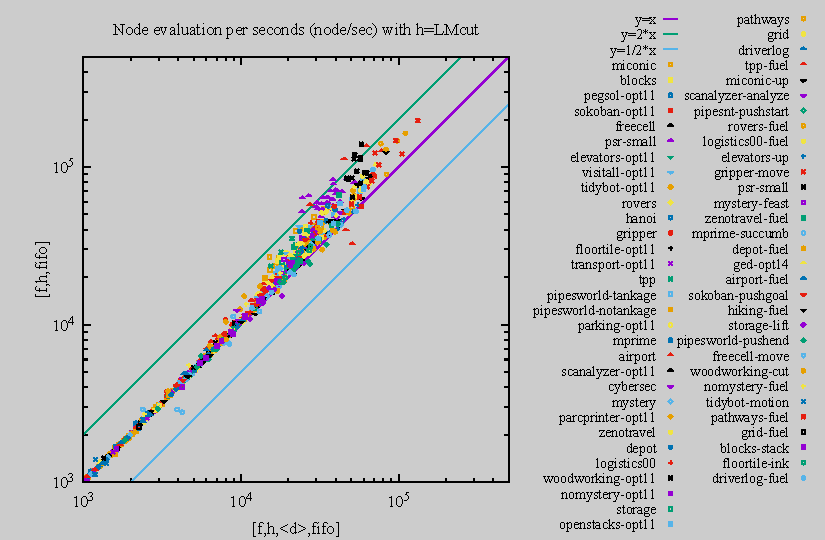
\includegraphics{img/node-sec/lmhiF-lmh_F.pdf}
 % % 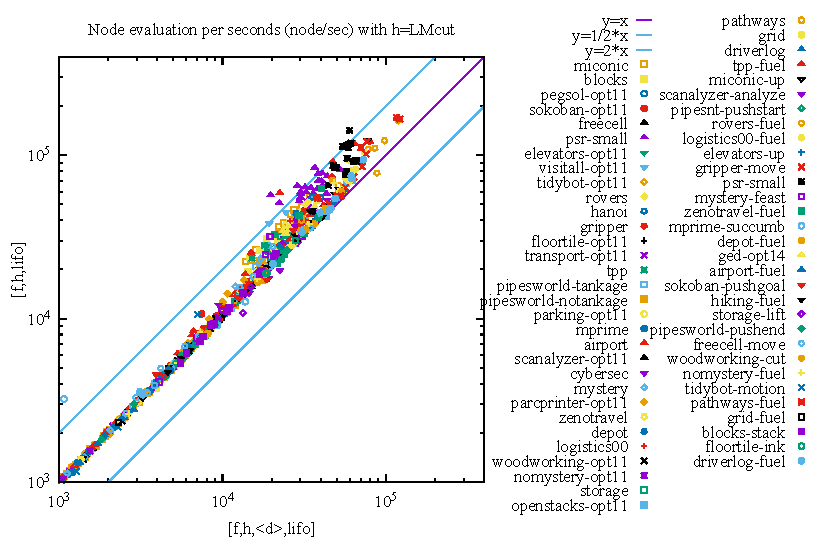
\includegraphics{img/node-sec/lmhiL-lmh_L.pdf}
 % 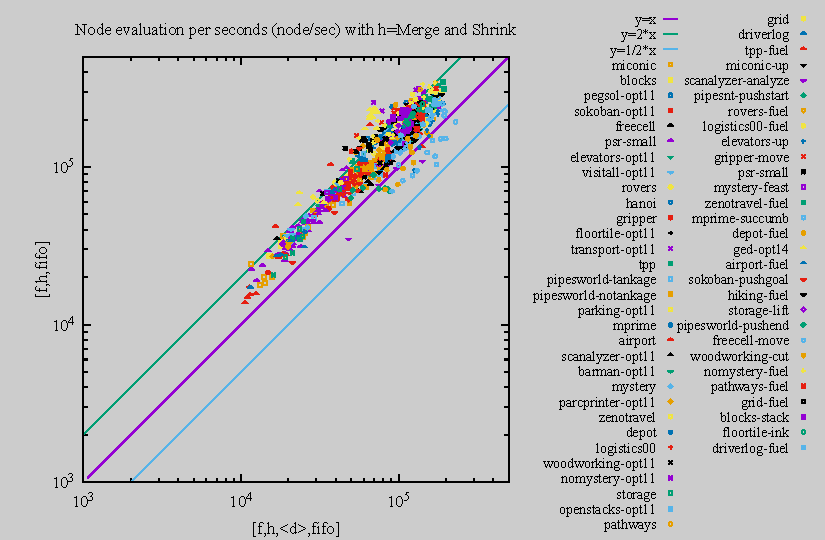
\includegraphics{img/node-sec/mnhiF-mnh_F.pdf}
 % % 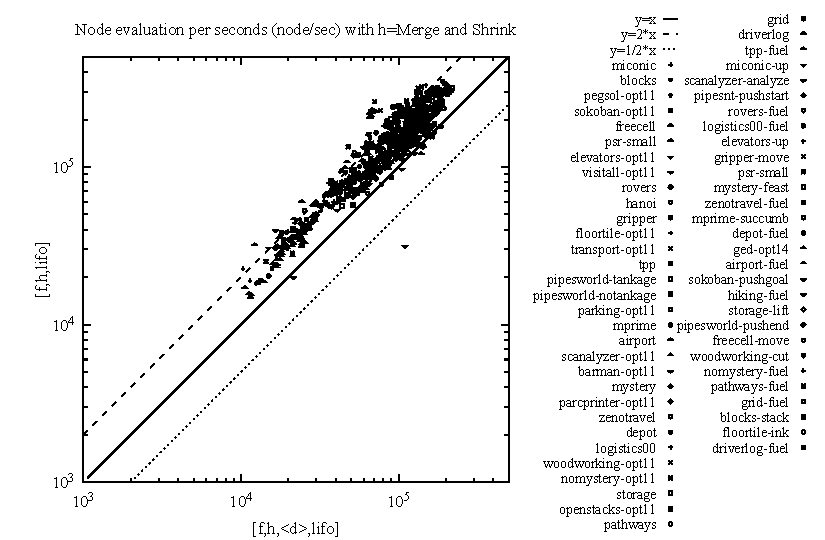
\includegraphics{img/node-sec/mnhiL-mnh_L.pdf}
 % 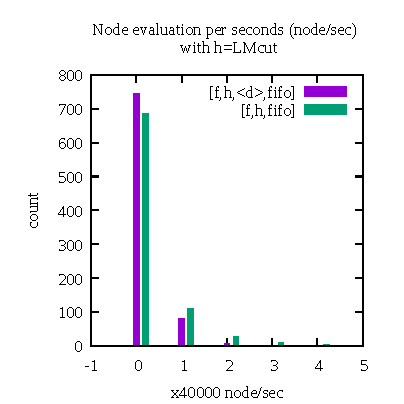
\includegraphics{img/node-sec/lmhiF-lmh_F-hist.pdf}
 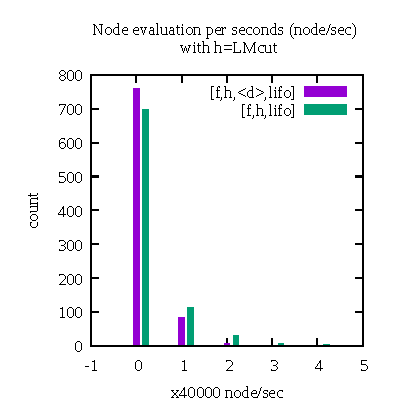
\includegraphics{img/node-sec/lmhiL-lmh_L-hist.pdf}
 % 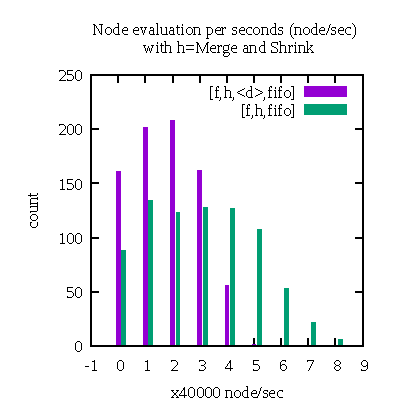
\includegraphics{img/node-sec/mnhiF-mnh_F-hist.pdf}
 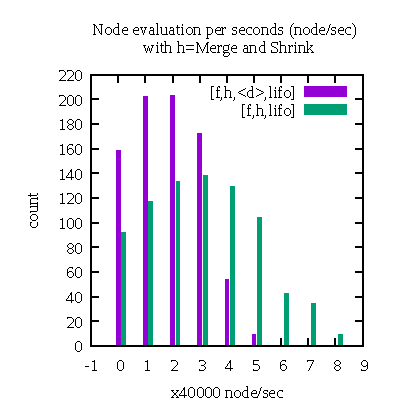
\includegraphics{img/node-sec/mnhiL-mnh_L-hist.pdf}
 % 
 \caption{Histogram comparing the node evaluation ratio (node/sec) between standard tie-breaking ($[f,h,\lifo]$) and
 depth-based tie-breaking ($[f,h,\depth,\lifo]$) on \lmcut and \mands heuristics.
 On \mands, compared to \lmcut, node evaluation rate more often becomes
 slower when depth is enabled. This is because the node evaluation of \mands is an order of
 magnitude faster than \lmcut, and the overhead of managing depth-based tie-breaking queue becomes significant.
 }
 % 
 \label{fig:expansion-ratio-lifo}
\end{figure}

% \clearpage
% \subsection{Additional Figures for \refig{fig:eval-comparison}: $\lifo$ Default Tiebreaking}
% 
% \begin{figure}[htbp]
%  \centering
%  % 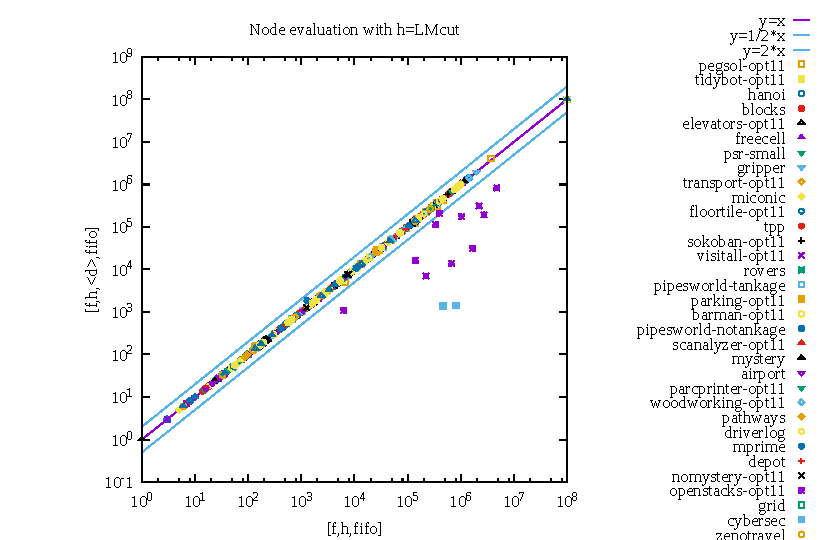
\includegraphics{img/node-sec/lmhiF-lmh_F-eval.pdf}
%  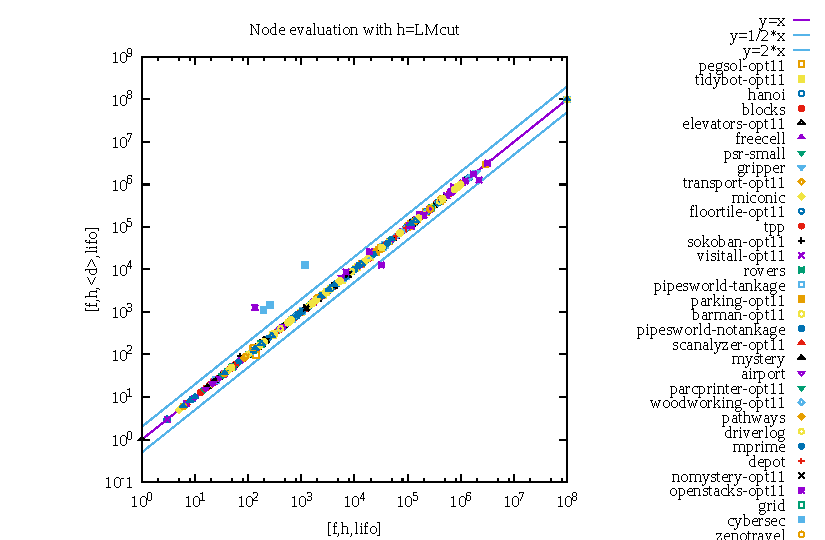
\includegraphics{img/node-sec/lmhiL-lmh_L-eval.pdf}
%  % 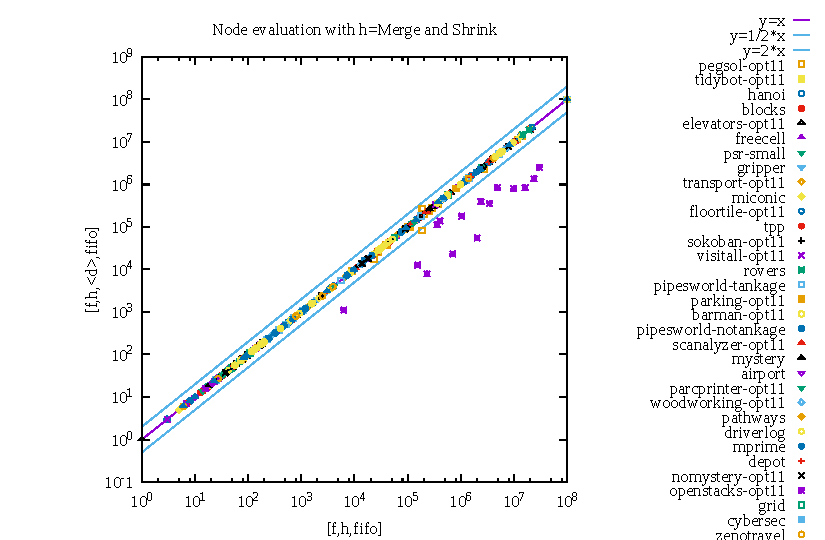
\includegraphics{img/node-sec/mnhiF-mnh_F-eval.pdf}
%  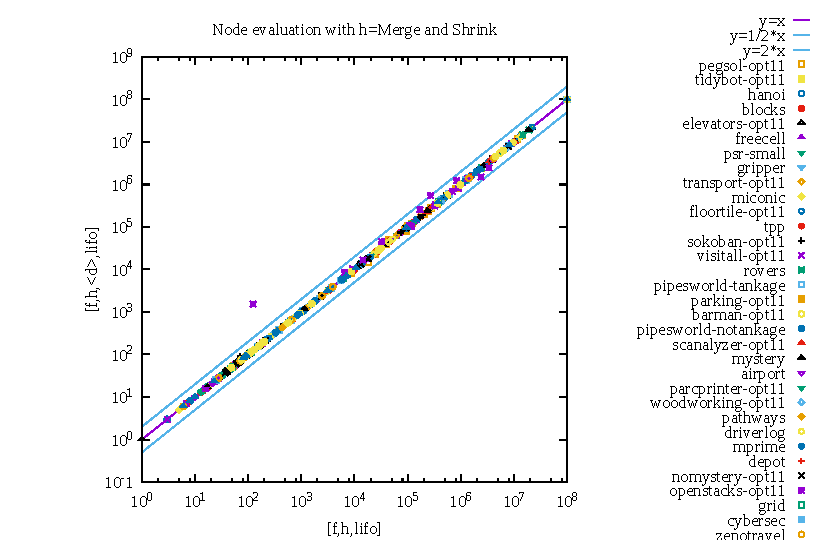
\includegraphics{img/node-sec/mnhiL-mnh_L-eval.pdf}
%  % \includegraphics{img/node-sec/lmhiF-lmh_F-exp.pdf}
%  % \includegraphics{img/node-sec/lmhiL-lmh_L-exp.pdf}
%  % \includegraphics{img/node-sec/mnhiF-mnh_F-exp.pdf}
%  % \includegraphics{img/node-sec/mnhiL-mnh_L-exp.pdf}
%  % 
%  \caption{Comparison of the number of evaluated nodes on IPC domains, between standard and depth-diversified search algorithms.
%  \pddl{Cybersec} and \pddl{Openstacks} shows that the evaluation is reduced by depth.
%  There are also slight effect on \pddl{pegsol-opt11} because it also contains zero-cost actions.
%  However, the two 0-cost actions (\pddl{jump-continue-move, end-move}) are the necessary ``finalization'' actions that should always be executed after the unit-cost action (\pddl{jump-start-move}).
%  Due to the characteristics of these actions, the effect of depth diversification on 0-cost actions are limited.
%  }
%  % 
%  \label{fig:eval-comparison-lifo}
% \end{figure}


\clearpage
\subsection{Additional Figures for \refig{fig:depth-histogram}: More Histograms for the Size of Final Plateaus}

These includes 12 additional histograms for the size of final plateaus on
more variety of domains and instances.

\begin{figure}[htbp]
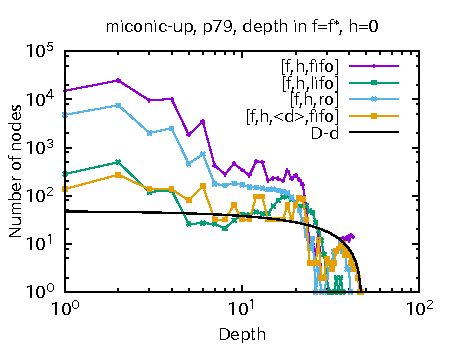
\includegraphics[width=0.49\linewidth]{img/output-lmcut/miconic-up/p79-0.pdf}
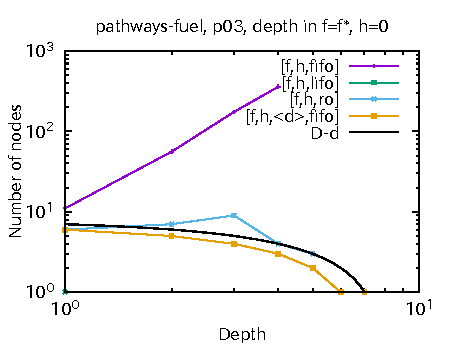
\includegraphics[width=0.49\linewidth]{img/output-lmcut/pathways-fuel/p03-0.pdf}
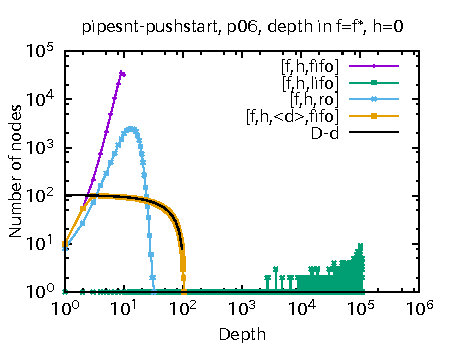
\includegraphics[width=0.49\linewidth]{img/output-lmcut/pipesnt-pushstart/p06-0.pdf}
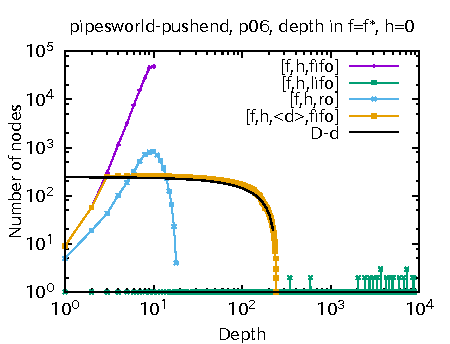
\includegraphics[width=0.49\linewidth]{img/output-lmcut/pipesworld-pushend/p06-0.pdf}
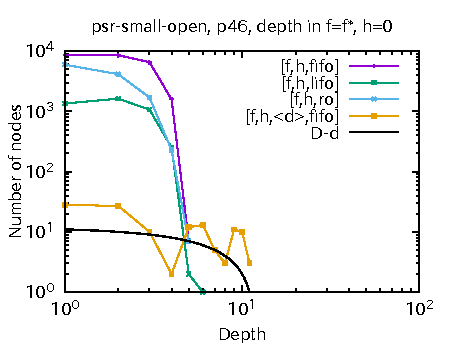
\includegraphics[width=0.49\linewidth]{img/output-lmcut/psr-small-open/p46-0.pdf}
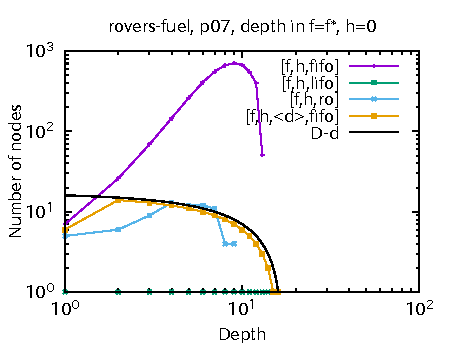
\includegraphics[width=0.49\linewidth]{img/output-lmcut/rovers-fuel/p07-0.pdf}
 \caption{(Page 1/2) Number of nodes ($y$-axis) expanded per depth ($x$-axis) in
 the final plateau with different tie-breaking strategies. Both axes are in logarithmic scale.
 }
 \label{fig:depth-histogram2}
\end{figure}

\begin{figure}[htbp]
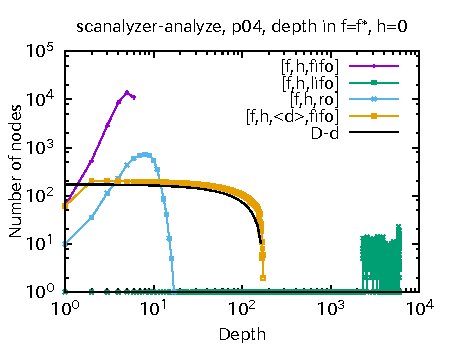
\includegraphics{img/output-lmcut/scanalyzer-analyze/p04-0.pdf}
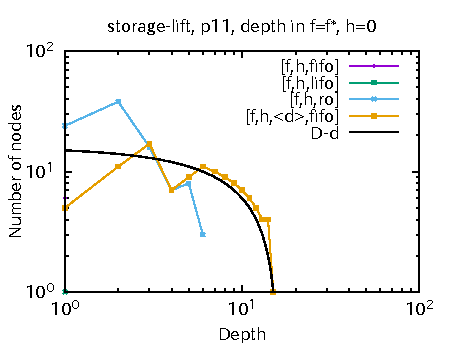
\includegraphics{img/output-lmcut/storage-lift/p11-0.pdf}
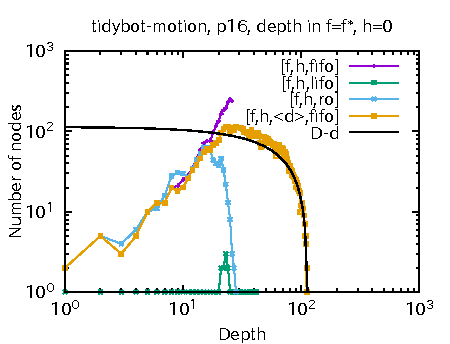
\includegraphics{img/output-lmcut/tidybot-motion/p16-0.pdf}
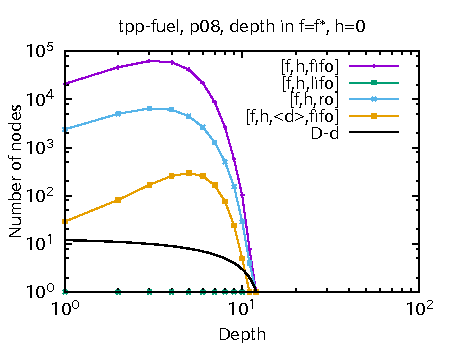
\includegraphics{img/output-lmcut/tpp-fuel/p08-0.pdf}
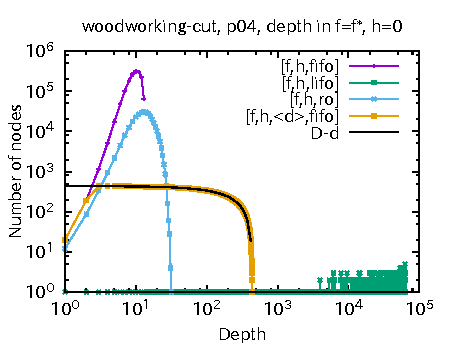
\includegraphics{img/output-lmcut/woodworking-cut/p04-0.pdf}
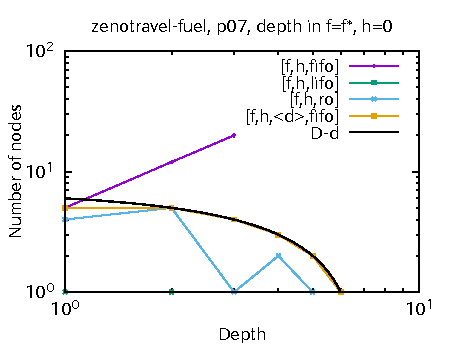
\includegraphics{img/output-lmcut/zenotravel-fuel/p07-0.pdf}
 \caption{(Page 2/2) Number of nodes ($y$-axis) expanded per depth ($x$-axis) in
 the final plateau with different tie-breaking strategies. Both axes are in logarithmic scale.
 }
 \label{fig:depth-histogram3}
\end{figure}

\clearpage
\subsection{Additional Figures for \refig{fig:depth-histogram4}: More Histograms for the Size of Non-Final Plateaus}

These are the additional histograms for the size of non-final plateaus on
more variety of domains and instances.

\begin{figure}[htbp]
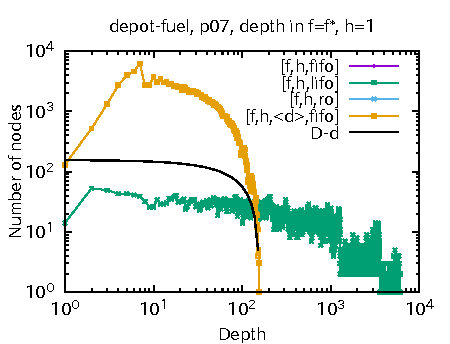
\includegraphics{img/output-lmcut/depot-fuel/p07-1.pdf}
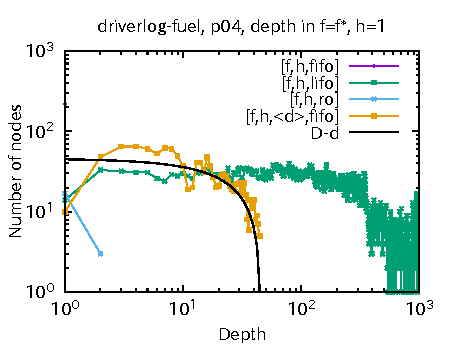
\includegraphics{img/output-lmcut/driverlog-fuel/p04-1.pdf}
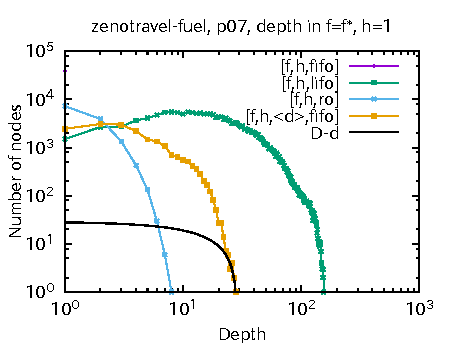
\includegraphics{img/output-lmcut/zenotravel-fuel/p07-1.pdf}
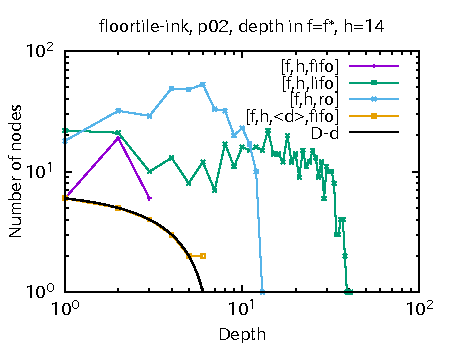
\includegraphics{img/output-lmcut/floortile-ink/p02-14.pdf}
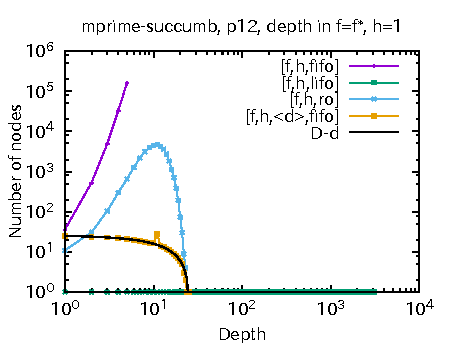
\includegraphics{img/output-lmcut/mprime-succumb/p12-1.pdf}
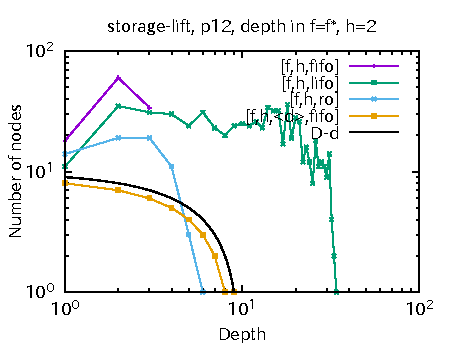
\includegraphics{img/output-lmcut/storage-lift/p12-2.pdf}
 \caption{Depth distribution in the non-final plateaus ($\plateau{f^*,h}, h\not=0$): Other domains.}
 \label{fig:depth-histogram5}
\end{figure}

\clearpage
\subsection{Detailed Data for \reftbl{tbl:dtg-summary}}

\setlength{\tabcolsep}{0.1em}

\begin{table}[htbp]
 {
 \relsize{-0.5}
 \centering
 \begin{center}
\begin{tabular}{|r|*{4}{ccc|}}
 & \rb{$[f,\hh,\fifo]$} & \rb{$[f,\hh,\lifo]$} & \rb{$[f,\hh,\ro]$} & \rb{$[f,h,\hh,\fifo]$} & \rb{$[f,h,\hh,\lifo]$} & \rb{$[f,h,\hh,\ro]$} & \rb{$[f,\ffo,\fifo]$} & \rb{$[f,\ffo,\lifo]$} & \rb{$[f,\ffo,\ro]$} & \rb{$[f,\ffo,\depth,\fifo]$} & \rb{$[f,\ffo,\depth,\lifo]$} & \rb{$[f,\ffo,\depth,\ro]$}\\
Zerocost (620) & 295 & 303 & 301.0 & 305 & 309 & 305.9 \(\pm\) 2.1 & 337 & 340 & 341 \(\pm\) 2.2 & 340 & 342 & \textbf{344.3} \(\pm\) 1.8\\
airport-fuel(20) & 13 & 12 & 12.7 & 14 & 12 & 12.8 \(\pm\) 0.8 & 13 & 11 & 11.7 \(\pm\) 0.5 & 13 & 11 & 11.7 \(\pm\) 0.5\\
blocks-stack(20) & 15 & 15 & 15.0 & 15 & 15 & 15 \(\pm\) 0 & 17 & 17 & 17 \(\pm\) 0 & 17 & 17 & 17 \(\pm\) 0\\
depot-fuel(22) & 6 & 6 & 6.0 & 6 & 6 & 6 \(\pm\) 0 & 6 & 6 & 6 \(\pm\) 0 & 6 & 6 & 6 \(\pm\) 0\\
driverlog-fuel(20) & 8 & 8 & 8.0 & 8 & 8 & 8 \(\pm\) 0 & 8 & 8 & 8 \(\pm\) 0 & 8 & 8 & 8 \(\pm\) 0\\
\textbf{elevators-up(20)} & \textbf{20} & \textbf{20} & 19.9 & \textbf{20} & \textbf{20} & \textbf{20} \(\pm\) 0 & \textbf{20} & \textbf{20} & \textbf{20} \(\pm\) 0 & \textbf{20} & \textbf{20} & \textbf{20} \(\pm\) 0\\
floortile-ink(20) & 8 & 8 & 8.0 & 8 & 8 & 8 \(\pm\) 0 & 9 & 8 & 8.7 \(\pm\) 0.5 & 9 & 8 & 8.7 \(\pm\) 0.5\\
freecell-move(20) & 12 & 14 & 13.3 & 12 & 14 & 13.2 \(\pm\) 0.4 & 17 & 18 & 17.9 \(\pm\) 0.8 & 17 & 18 & 18.3 \(\pm\) 0.9\\
grid-fuel(5) & 1 & 1 & 1.0 & 1 & 1 & 1 \(\pm\) 0 & 1 & 1 & 1 \(\pm\) 0 & 1 & 1 & 1 \(\pm\) 0\\
gripper-move(20) & 6 & 6 & 6.0 & 6 & 6 & 6 \(\pm\) 0 & 6 & 6 & 6 \(\pm\) 0 & 6 & 6 & 6 \(\pm\) 0\\
hiking-fuel(20) & 8 & 8 & 8.0 & 8 & 8 & 8 \(\pm\) 0 & 9 & 9 & 9 \(\pm\) 0 & 9 & 9 & 9 \(\pm\) 0\\
logistics00-fuel(28) & 15 & 15 & 15.0 & 15 & 15 & 15 \(\pm\) 0 & 15 & 15 & 15 \(\pm\) 0 & 15 & 15 & 15 \(\pm\) 0\\
\textbf{miconic-up(30)} & 14 & 17 & 15.1 & 14 & 17 & 15.1 \(\pm\) 0.9 & 15 & \textbf{21} & 17.9 \(\pm\) 1.2 & 15 & \textbf{21} & 18 \(\pm\) 1.2\\
\textbf{mprime-succumb(35)} & 19 & 16 & 19.1 & 20 & 16 & 20.1 \(\pm\) 0.6 & \textbf{30} & 23 & 28.3 \(\pm\) 0.9 & \textbf{30} & 27 & 29.3 \(\pm\) 0.7\\
\textbf{mystery-feast(20)} & 7 & 6 & 6.9 & 6 & 5 & 5.9 \(\pm\) 0.3 & \textbf{8} & \textbf{8} & \textbf{8} \(\pm\) 0 & \textbf{8} & \textbf{8} & \textbf{8} \(\pm\) 0\\
nomystery-fuel(20) & 10 & 10 & 10.0 & 10 & 10 & 10 \(\pm\) 0 & 10 & 10 & 10 \(\pm\) 0 & 10 & 10 & 10 \(\pm\) 0\\
\textbf{parking-movecc(20)} & 13 & 14 & 14.3 & 13 & 15 & 14.4 \(\pm\) 1.5 & \textbf{20} & \textbf{20} & \textbf{20} \(\pm\) 0 & \textbf{20} & \textbf{20} & \textbf{20} \(\pm\) 0\\
pathways-fuel(30) & 5 & 5 & 4.1 & 5 & 5 & 4 \(\pm\) 0 & 5 & 5 & 5 \(\pm\) 0 & 5 & 5 & 5 \(\pm\) 0\\
pipesnt-pushstart(20) & 7 & 8 & 7.7 & 8 & 8 & 7.8 \(\pm\) 0.4 & 9 & 9 & 9 \(\pm\) 0 & 9 & 9 & 9 \(\pm\) 0\\
\textbf{pipesworld-pushend(20)} & 5 & 6 & 5.1 & 5 & 5 & 5 \(\pm\) 0 & 7 & \textbf{8} & 7.1 \(\pm\) 0.3 & 7 & 7 & 7.7 \(\pm\) 0.5\\
psr-small-open(20) & 19 & 19 & 19.0 & 19 & 19 & 19 \(\pm\) 0 & 19 & 19 & 19 \(\pm\) 0 & 19 & 19 & 19 \(\pm\) 0\\
rovers-fuel(40) & 7 & 7 & 7.0 & 7 & 7 & 7 \(\pm\) 0 & 8 & 9 & 8 \(\pm\) 0 & 8 & 8 & 8 \(\pm\) 0\\
\textbf{scanalyzer-analyze(20)} & 8 & 11 & 10.1 & 16 & \textbf{18} & 15.3 \(\pm\) 0.9 & 15 & 15 & 15 \(\pm\) 0 & 15 & 15 & 15 \(\pm\) 0\\
sokoban-pushgoal(20) & 16 & 16 & 16.0 & 16 & 16 & 16 \(\pm\) 0 & 17 & 17 & 17 \(\pm\) 0 & 17 & 17 & 17 \(\pm\) 0\\
storage-lift(20) & 4 & 4 & 4.0 & 4 & 4 & 4 \(\pm\) 0 & 4 & 4 & 4.3 \(\pm\) 0.5 & 4 & 4 & 4.8 \(\pm\) 0.4\\
tidybot-motion(20) & 14 & 14 & 14.0 & 14 & 14 & 14 \(\pm\) 0 & 15 & 16 & 16 \(\pm\) 0 & 16 & 16 & 15.9 \(\pm\) 0.3\\
tpp-fuel(30) & 8 & 10 & 8.7 & 8 & 10 & 8.2 \(\pm\) 0.4 & 8 & 10 & 9.1 \(\pm\) 0.3 & 10 & 10 & 10 \(\pm\) 0\\
\textbf{woodworking-cut(20)} & \textbf{20} & \textbf{20} & \textbf{20.0} & \textbf{20} & \textbf{20} & \textbf{20} \(\pm\) 0 & 19 & \textbf{20} & \textbf{20} \(\pm\) 0 & 19 & \textbf{20} & \textbf{20} \(\pm\) 0\\
zenotravel-fuel(20) & 7 & 7 & 7.0 & 7 & 7 & 7 \(\pm\) 0 & 7 & 7 & 7 \(\pm\) 0 & 7 & 7 & 7 \(\pm\) 0\\
\end{tabular}
\end{center}

 \caption{
 Coverage results with { \lmcut for computing $f$ and inadmissible distance-to-go heuristics for tie-breaking, on 620 Zerocost instances}. We highlight the best results when the difference between the maximum and the minimum coverage exceeds 2, over all configurations \emph{including \reftbl{tbl:lmcut-zerocost-full}}.
 }
 \label{tbl:dtg-lmcut-zero}
 }
\end{table}

\begin{table}[htbp]
 {
 \relsize{-0.5}
 \centering
 \let\hline\midrule
\begin{center}
\begin{tabular}{|r|*{4}{ccc|}}
 & \rb{$[f,\hh,\fifo]$} & \rb{$[f,\hh,\lifo]$} & \rb{$[f,\hh,\ro]$} & \rb{$[f,h,\hh,\fifo]$} & \rb{$[f,h,\hh,\lifo]$} & \rb{$[f,h,\hh,\ro]$} & \rb{$[f,\ffo,\fifo]$} & \rb{$[f,\ffo,\lifo]$} & \rb{$[f,\ffo,\ro]$} & \rb{$[f,\ffo,\depth,\fifo]$} & \rb{$[f,\ffo,\depth,\lifo]$} & \rb{$[f,\ffo,\depth,\ro]$}\\
Zerocost (620) & 308 & 305 & 307.3 \(\pm\) 1.5 & 307 & 306 & 307.8 \(\pm\) 1.4 & 336 & 331 & \textbf{337.9} \(\pm\) 2.1 & 337 & 333 & 337.6 \(\pm\) 1.3\\
\hline
airport-fuel(20) & 1 & 1 & 1 \(\pm\) 0 & 1 & 1 & 1 \(\pm\) 0 & 5 & 5 & 5 \(\pm\) 0 & 5 & 5 & 5 \(\pm\) 0\\
blocks-stack(20) & 20 & 20 & 20 \(\pm\) 0 & 20 & 20 & 20 \(\pm\) 0 & 20 & 19 & 19.9 \(\pm\) 0.3 & 20 & 20 & 19.9 \(\pm\) 0.3\\
depot-fuel(22) & 6 & 6 & 6 \(\pm\) 0 & 6 & 6 & 6 \(\pm\) 0 & 4 & 4 & 4 \(\pm\) 0 & 4 & 4 & 4 \(\pm\) 0\\
driverlog-fuel(20) & 9 & 9 & 9 \(\pm\) 0 & 9 & 9 & 9 \(\pm\) 0 & 9 & 9 & 9 \(\pm\) 0 & 9 & 9 & 9 \(\pm\) 0\\
\textbf{elevators-up(20)} & 19 & 19 & 19 \(\pm\) 0 & 19 & 19 & 19 \(\pm\) 0 & \textbf{20} & \textbf{20} & \textbf{20} \(\pm\) 0 & \textbf{20} & \textbf{20} & \textbf{20} \(\pm\) 0\\
floortile-ink(20) & 8 & 8 & 8 \(\pm\) 0 & 8 & 8 & 8 \(\pm\) 0 & 9 & 8 & 8.8 \(\pm\) 0.4 & 9 & 8 & 8.8 \(\pm\) 0.4\\
freecell-move(20) & 13 & 14 & 12.7 \(\pm\) 0.7 & 13 & 13 & 12.7 \(\pm\) 0.7 & 17 & 17 & 17.4 \(\pm\) 0.5 & 17 & 17 & 17.3 \(\pm\) 0.7\\
grid-fuel(5) & 2 & 2 & 2 \(\pm\) 0 & 2 & 2 & 2 \(\pm\) 0 & 2 & 2 & 2 \(\pm\) 0 & 2 & 2 & 2 \(\pm\) 0\\
gripper-move(20) & 20 & 20 & 20 \(\pm\) 0 & 20 & 20 & 20 \(\pm\) 0 & 20 & 20 & 20 \(\pm\) 0 & 20 & 20 & 20 \(\pm\) 0\\
hiking-fuel(20) & 13 & 13 & 12.1 \(\pm\) 0.3 & 13 & 13 & 12.1 \(\pm\) 0.3 & 11 & 11 & 11 \(\pm\) 0 & 11 & 11 & 11 \(\pm\) 0\\
logistics00-fuel(28) & 16 & 16 & 16 \(\pm\) 0 & 16 & 16 & 16 \(\pm\) 0 & 16 & 16 & 16 \(\pm\) 0 & 16 & 16 & 16 \(\pm\) 0\\
miconic-up(30) & 22 & 22 & 22 \(\pm\) 0 & 22 & 22 & 22.1 \(\pm\) 0.3 & 30 & 30 & 30 \(\pm\) 0 & 30 & 30 & 30 \(\pm\) 0\\
\textbf{mprime-succumb(35)} & 21 & 17 & 20.4 \(\pm\) 0.7 & 21 & 17 & 20.4 \(\pm\) 0.7 & \textbf{28} & 23 & 27.4 \(\pm\) 0.7 & \textbf{28} & 25 & 27.7 \(\pm\) 0.7\\
mystery-feast(20) & 5 & 5 & 5 \(\pm\) 0 & 5 & 5 & 5 \(\pm\) 0 & 3 & 3 & 3 \(\pm\) 0 & 3 & 3 & 3 \(\pm\) 0\\
nomystery-fuel(20) & 16 & 16 & 16 \(\pm\) 0 & 16 & 16 & 16 \(\pm\) 0 & 15 & 15 & 15 \(\pm\) 0 & 15 & 15 & 15 \(\pm\) 0\\
\textbf{parking-movecc(20)} & 2 & 2 & 2 \(\pm\) 0 & 2 & 2 & 2 \(\pm\) 0 & 10 & 10 & \textbf{10.3} \(\pm\) 1.0 & 10 & 10 & \textbf{10.3} \(\pm\) 1.0\\
pathways-fuel(30) & 4 & 4 & 4 \(\pm\) 0 & 4 & 4 & 4 \(\pm\) 0 & 4 & 4 & 4 \(\pm\) 0 & 4 & 4 & 4 \(\pm\) 0\\
pipesnt-pushstart(20) & 1 & 2 & 1.9 \(\pm\) 0.8 & 1 & 2 & 1.8 \(\pm\) 0.7 & 5 & 5 & 5 \(\pm\) 0 & 5 & 5 & 5 \(\pm\) 0\\
pipesworld-pushend(20) & 8 & 7 & 7.8 \(\pm\) 0.4 & 8 & 8 & 8 \(\pm\) 0 & 5 & 5 & 5.4 \(\pm\) 0.7 & 5 & 5 & 5.6 \(\pm\) 0.5\\
psr-small-open(20) & 19 & 19 & 19 \(\pm\) 0 & 19 & 19 & 19 \(\pm\) 0 & 19 & 19 & 19 \(\pm\) 0 & 19 & 19 & 19 \(\pm\) 0\\
rovers-fuel(40) & 8 & 8 & 8 \(\pm\) 0 & 8 & 8 & 8 \(\pm\) 0 & 8 & 8 & 8 \(\pm\) 0 & 8 & 8 & 8 \(\pm\) 0\\
\textbf{scanalyzer-analyze(20)} & 15 & 14 & 15 \(\pm\) 0 & 14 & 15 & 15 \(\pm\) 0 & 15 & 16 & \textbf{15.4} \(\pm\) 0.7 & 15 & 15 & 15.2 \(\pm\) 0.7\\
sokoban-pushgoal(20) & 17 & 17 & 17 \(\pm\) 0 & 17 & 17 & 17 \(\pm\) 0 & 18 & 18 & 18.2 \(\pm\) 0.4 & 18 & 18 & 18 \(\pm\) 0\\
storage-lift(20) & 4 & 4 & 4 \(\pm\) 0 & 4 & 4 & 4 \(\pm\) 0 & 4 & 4 & 4 \(\pm\) 0 & 4 & 4 & 4 \(\pm\) 0\\
tidybot-motion(20) & 0 & 0 & 0 \(\pm\) 0 & 0 & 0 & 0 \(\pm\) 0 & 0 & 0 & 0 \(\pm\) 0 & 0 & 0 & 0 \(\pm\) 0\\
tpp-fuel(30) & 9 & 10 & 9.4 \(\pm\) 0.5 & 9 & 10 & 9.8 \(\pm\) 0.4 & 10 & 11 & 10.9 \(\pm\) 0.3 & 11 & 11 & 10.9 \(\pm\) 0.3\\
\textbf{woodworking-cut(20)} & \textbf{20} & \textbf{20} & \textbf{20} \(\pm\) 0 & \textbf{20} & \textbf{20} & \textbf{20} \(\pm\) 0 & \textbf{20} & \textbf{20} & \textbf{20} \(\pm\) 0 & \textbf{20} & \textbf{20} & \textbf{20} \(\pm\) 0\\
zenotravel-fuel(20) & 10 & 10 & 10 \(\pm\) 0 & 10 & 10 & 9.9 \(\pm\) 0.3 & 9 & 9 & 9 \(\pm\) 0 & 9 & 9 & 8.9 \(\pm\) 0.3\\
\end{tabular}
\end{center}

 \caption{
 Coverage results with \mands for computing $f$ and inadmissible distance-to-go heuristics for tie-breaking, on 620 Zerocost instances. We highlight the best results when the difference between the maximum and the minimum coverage exceeds 2, over all configurations \emph{including \reftbl{tbl:mands-zerocost-full}}.
 }
 \label{tbl:dtg-mands-zero}
 }
\end{table}

\begin{table}[htbp]
 {
 \relsize{-0.5} 
 \centering
 \let\hline\midrule
\begin{center}
\begin{tabular}{|r|*{4}{ccc|}}
 & \rb{$[f,\hh,\fifo]$} & \rb{$[f,\hh,\lifo]$} & \rb{$[f,\hh,\ro]$} & \rb{$[f,h,\hh,\fifo]$} & \rb{$[f,h,\hh,\lifo]$} & \rb{$[f,h,\hh,\ro]$} & \rb{$[f,\ffo,\fifo]$} & \rb{$[f,\ffo,\lifo]$} & \rb{$[f,\ffo,\ro]$} & \rb{$[f,\ffo,\depth,\fifo]$} & \rb{$[f,\ffo,\depth,\lifo]$} & \rb{$[f,\ffo,\depth,\ro]$}\\
IPC benchmark (1104) & 534 & 534 & 534 $\pm$ 2.1 & 536 & 535 & 534.7 $\pm$ 1.5 & 564 & 562 & 563.7 $\pm$ 1.4 & 563 & 560 & 561.9 $\pm$ 1.4\\
\hline
airport(50) & 24 & 25 & 23.9 $\pm$ 0.6 & 24 & 24 & 23.8 $\pm$ 0.4 & 25 & 24 & 24.8 $\pm$ 0.4 & 25 & 24 & 24.6 $\pm$ 0.5\\
barman-opt11(20) & 0 & 0 & 0 $\pm$ 0 & 0 & 0 & 0 $\pm$ 0 & 0 & 0 & 0 $\pm$ 0 & 0 & 0 & 0 $\pm$ 0\\
blocks(35) & 27 & 27 & 27 $\pm$ 0 & 27 & 27 & 27 $\pm$ 0 & 27 & 27 & 27 $\pm$ 0 & 27 & 27 & 27 $\pm$ 0\\
cybersec(19) & 5 & 3 & 5.9 $\pm$ 1.2 & 6 & 4 & 5.4 $\pm$ 0.7 & 6 & 6 & 5.9 $\pm$ 0.8 & 6 & 5 & 5.6 $\pm$ 0.7\\
depot(22) & 5 & 5 & 5 $\pm$ 0 & 5 & 5 & 5 $\pm$ 0 & 6 & 6 & 6 $\pm$ 0 & 6 & 6 & 6 $\pm$ 0\\
driverlog(20) & 12 & 12 & 12 $\pm$ 0 & 12 & 12 & 12 $\pm$ 0 & 13 & 13 & 13 $\pm$ 0 & 13 & 13 & 13 $\pm$ 0\\
elevators-opt11(20) & 12 & 12 & 12 $\pm$ 0 & 12 & 12 & 12 $\pm$ 0 & 15 & 15 & 14.9 $\pm$ 0.3 & 14 & 15 & 14 $\pm$ 0\\
floortile-opt11(20) & 6 & 6 & 6 $\pm$ 0 & 6 & 6 & 6 $\pm$ 0 & 6 & 6 & 6 $\pm$ 0 & 6 & 6 & 6 $\pm$ 0\\
freecell(80) & 8 & 8 & 8 $\pm$ 0 & 8 & 8 & 8 $\pm$ 0 & 9 & 9 & 9 $\pm$ 0 & 9 & 9 & 9 $\pm$ 0\\
grid(5) & 1 & 1 & 1 $\pm$ 0 & 1 & 1 & 1 $\pm$ 0 & 1 & 1 & 1 $\pm$ 0 & 1 & 1 & 1 $\pm$ 0\\
gripper(20) & 6 & 6 & 6 $\pm$ 0 & 6 & 6 & 6 $\pm$ 0 & 6 & 6 & 6 $\pm$ 0 & 6 & 6 & 6 $\pm$ 0\\
hanoi(30) & 11 & 11 & 11 $\pm$ 0 & 11 & 11 & 11 $\pm$ 0 & 12 & 12 & 12 $\pm$ 0 & 12 & 12 & 11.9 $\pm$ 0.3\\
logistics00(28) & 17 & 17 & 17 $\pm$ 0 & 17 & 17 & 17 $\pm$ 0 & 20 & 20 & 20 $\pm$ 0 & 20 & 20 & 20 $\pm$ 0\\
miconic(150) & 140 & 140 & 140 $\pm$ 0 & 140 & 140 & 140 $\pm$ 0 & 140 & 140 & 140 $\pm$ 0 & 140 & 140 & 140 $\pm$ 0\\
mprime(35) & 20 & 21 & 19.9 $\pm$ 0.8 & 20 & 21 & 20 $\pm$ 0.7 & 22 & 22 & 22 $\pm$ 0 & 22 & 22 & 22 $\pm$ 0\\
mystery(30) & 15 & 15 & 15 $\pm$ 0 & 15 & 15 & 15 $\pm$ 0 & 16 & 16 & 16 $\pm$ 0 & 16 & 16 & 16 $\pm$ 0\\
nomystery-opt11(20) & 13 & 13 & 13 $\pm$ 0 & 13 & 13 & 13 $\pm$ 0 & 14 & 14 & 14 $\pm$ 0 & 14 & 14 & 14 $\pm$ 0\\
openstacks-opt11(20) & 10 & 10 & 10 $\pm$ 0 & 10 & 10 & 9.9 $\pm$ 0.3 & 17 & 17 & 17 $\pm$ 0 & 17 & 17 & 17 $\pm$ 0\\
parcprinter-opt11(20) & 13 & 13 & 13 $\pm$ 0 & 13 & 13 & 13 $\pm$ 0 & 13 & 13 & 13 $\pm$ 0 & 13 & 13 & 13 $\pm$ 0\\
parking-opt11(20) & 1 & 1 & 1 $\pm$ 0 & 1 & 1 & 1 $\pm$ 0 & 1 & 1 & 1 $\pm$ 0 & 1 & 1 & 1 $\pm$ 0\\
pathways(30) & 5 & 5 & 5 $\pm$ 0 & 5 & 5 & 5 $\pm$ 0 & 5 & 5 & 5 $\pm$ 0 & 5 & 5 & 5 $\pm$ 0\\
pegsol-opt11(20) & 16 & 16 & 16 $\pm$ 0 & 16 & 16 & 16 $\pm$ 0 & 17 & 17 & 17 $\pm$ 0 & 17 & 17 & 17 $\pm$ 0\\
pipesworld-notankage(50) & 12 & 12 & 12 $\pm$ 0 & 12 & 12 & 12 $\pm$ 0 & 13 & 13 & 13 $\pm$ 0 & 13 & 13 & 13 $\pm$ 0\\
pipesworld-tankage(50) & 7 & 7 & 7 $\pm$ 0 & 7 & 7 & 7 $\pm$ 0 & 8 & 8 & 8 $\pm$ 0 & 8 & 8 & 8 $\pm$ 0\\
psr-small(50) & 48 & 48 & 47.9 $\pm$ 0.3 & 48 & 48 & 48 $\pm$ 0 & 48 & 48 & 48 $\pm$ 0 & 48 & 48 & 48 $\pm$ 0\\
rovers(40) & 7 & 7 & 7 $\pm$ 0 & 7 & 7 & 7 $\pm$ 0 & 7 & 7 & 7 $\pm$ 0 & 7 & 7 & 7 $\pm$ 0\\
scanalyzer-opt11(20) & 8 & 10 & 8.8 $\pm$ 0.4 & 10 & 10 & 10 $\pm$ 0 & 10 & 10 & 10 $\pm$ 0 & 10 & 10 & 10 $\pm$ 0\\
sokoban-opt11(20) & 17 & 17 & 17 $\pm$ 0 & 17 & 17 & 17 $\pm$ 0 & 19 & 19 & 19 $\pm$ 0 & 19 & 19 & 19 $\pm$ 0\\
storage(30) & 14 & 14 & 14 $\pm$ 0 & 14 & 14 & 14 $\pm$ 0 & 14 & 14 & 14 $\pm$ 0 & 14 & 14 & 14 $\pm$ 0\\
tidybot-opt11(20) & 10 & 11 & 10.3 $\pm$ 0.5 & 11 & 11 & 10.6 $\pm$ 0.5 & 11 & 11 & 11 $\pm$ 0 & 11 & 11 & 11 $\pm$ 0\\
tpp(30) & 6 & 6 & 6 $\pm$ 0 & 6 & 6 & 6 $\pm$ 0 & 6 & 6 & 6 $\pm$ 0 & 6 & 6 & 6 $\pm$ 0\\
transport-opt11(20) & 6 & 6 & 6 $\pm$ 0 & 6 & 6 & 6 $\pm$ 0 & 6 & 6 & 6 $\pm$ 0 & 6 & 6 & 6 $\pm$ 0\\
visitall-opt11(20) & 10 & 10 & 10 $\pm$ 0 & 10 & 10 & 10 $\pm$ 0 & 10 & 10 & 10 $\pm$ 0 & 10 & 10 & 10 $\pm$ 0\\
woodworking-opt11(20) & 11 & 8 & 9.3 $\pm$ 1.0 & 9 & 9 & 9 $\pm$ 0 & 10 & 9 & 10.1 $\pm$ 1.1 & 10 & 8 & 9.9 $\pm$ 1.1\\
zenotravel(20) & 11 & 11 & 11 $\pm$ 0 & 11 & 11 & 11 $\pm$ 0 & 11 & 11 & 11 $\pm$ 0 & 11 & 11 & 11 $\pm$ 0\\
\end{tabular}
\end{center}

 \caption{
 Coverage results with \lmcut for computing $f$ and inadmissible distance-to-go heuristics for tie-breaking, on 1104 standard IPC benchmark instances.
 }
 \label{tbl:dtg-lmcut-ipc}
 }
\end{table}

\begin{table}[htbp]
 {
 \relsize{-0.5}
 \centering
 \begin{center}
\begin{tabular}{|r|cccHHH|cccHHH|cccHHH|cccHHH|cccHHH|}
Domain & $[f,\ffo,\fifo]$ & $[f,\ffo,\lifo]$ & $[f,\ffo,\ro]$ & R & R & R & $[f,\ffo,\depth,\fifo]$ & $[f,\ffo,\depth,\lifo]$ & $[f,\ffo,\depth,\ro]$ & R & R & R & $[f,\gco,\fifo]$ & $[f,\gco,\lifo]$ & $[f,\gco,\ro]$ & R & R & R & $[f,h,\hat{h},\depth,\fifo]$ & $[f,h,\hat{h},\depth,\lifo]$ & $[f,h,\hat{h},\depth,\ro]$ & R & R & R & $[f,\hat{h},\depth,\fifo]$ & $[f,\hat{h},\depth,\lifo]$ & $[f,\hat{h},\depth,\ro]$ & R & R & R\\
\hline
IPC benchmark (1104) & 458 & 457 & 456.3 $\pm$ 0.6 & 456 & 457 & 456 & 457 & 457 & 456 $\pm$ 1 & 455 & 457 & 456 & 494 & 495 & 490.3 $\pm$ 1.5 & 492 & 489 & 490 & 476 & 475 & 471.3 $\pm$ 0.6 & 472 & 471 & 471 & 477 & 475 & 471 $\pm$ 1 & 471 & 470 & 472\\
\hline
airport(50) & 9 & 9 & 9 $\pm$ 0 & 9 & 9 & 9 & 9 & 9 & 9 $\pm$ 0 & 9 & 9 & 9 & 9 & 9 & 9 $\pm$ 0 & 9 & 9 & 9 & 7 & 7 & 7 $\pm$ 0 & 7 & 7 & 7 & 7 & 7 & 7 $\pm$ 0 & 7 & 7 & 7\\
barman-opt11(20) & 4 & 4 & 4 $\pm$ 0 & 4 & 4 & 4 & 4 & 4 & 4 $\pm$ 0 & 4 & 4 & 4 & 4 & 4 & 4 $\pm$ 0 & 4 & 4 & 4 & 4 & 4 & 4 $\pm$ 0 & 4 & 4 & 4 & 4 & 4 & 4 $\pm$ 0 & 4 & 4 & 4\\
blocks(35) & 21 & 20 & 20 $\pm$ 0 & 20 & 20 & 20 & 20 & 20 & 20 $\pm$ 0 & 20 & 20 & 20 & 22 & 22 & 22 $\pm$ 0 & 22 & 22 & 22 & 21 & 21 & 21 $\pm$ 0 & 21 & 21 & 21 & 22 & 21 & 21 $\pm$ 0 & 21 & 21 & 21\\
\textbf{cybersec(19)} & 0 & 0 & 0 $\pm$ 0 & 0 & 0 & 0 & 0 & 0 & 0 $\pm$ 0 & 0 & 0 & 0 & 0 & 0 & 0 $\pm$ 0 & 0 & 0 & 0 & 0 & 0 & 0 $\pm$ 0 & 0 & 0 & 0 & 0 & 0 & 0 $\pm$ 0 & 0 & 0 & 0\\
depot(22) & 4 & 4 & 4 $\pm$ 0 & 4 & 4 & 4 & 4 & 4 & 4 $\pm$ 0 & 4 & 4 & 4 & 5 & 6 & 5 $\pm$ 0 & 5 & 5 & 5 & 5 & 5 & 5 $\pm$ 0 & 5 & 5 & 5 & 5 & 5 & 5 $\pm$ 0 & 5 & 5 & 5\\
driverlog(20) & 11 & 11 & 11 $\pm$ 0 & 11 & 11 & 11 & 11 & 11 & 11 $\pm$ 0 & 11 & 11 & 11 & 12 & 12 & 12 $\pm$ 0 & 12 & 12 & 12 & 12 & 12 & 12 $\pm$ 0 & 12 & 12 & 12 & 12 & 12 & 12 $\pm$ 0 & 12 & 12 & 12\\
elevators-opt11(20) & 10 & 10 & 10 $\pm$ 0 & 10 & 10 & 10 & 10 & 10 & 10 $\pm$ 0 & 10 & 10 & 10 & 13 & 13 & 13 $\pm$ 0 & 13 & 13 & 13 & 13 & 13 & 12 $\pm$ 0 & 12 & 12 & 12 & 13 & 13 & 12 $\pm$ 0 & 12 & 12 & 12\\
floortile-opt11(20) & 7 & 7 & 7 $\pm$ 0 & 7 & 7 & 7 & 7 & 7 & 7 $\pm$ 0 & 7 & 7 & 7 & 6 & 6 & 6 $\pm$ 0 & 6 & 6 & 6 & 6 & 6 & 6 $\pm$ 0 & 6 & 6 & 6 & 6 & 6 & 6 $\pm$ 0 & 6 & 6 & 6\\
freecell(80) & 14 & 14 & 14 $\pm$ 0 & 14 & 14 & 14 & 14 & 14 & 14 $\pm$ 0 & 14 & 14 & 14 & 17 & 17 & 16 $\pm$ 0 & 16 & 16 & 16 & 15 & 15 & 15 $\pm$ 0 & 15 & 15 & 15 & 15 & 15 & 15 $\pm$ 0 & 15 & 15 & 15\\
grid(5) & 2 & 2 & 2 $\pm$ 0 & 2 & 2 & 2 & 2 & 2 & 2 $\pm$ 0 & 2 & 2 & 2 & 2 & 2 & 2 $\pm$ 0 & 2 & 2 & 2 & 2 & 2 & 2 $\pm$ 0 & 2 & 2 & 2 & 2 & 2 & 2 $\pm$ 0 & 2 & 2 & 2\\
gripper(20) & 20 & 20 & 20 $\pm$ 0 & 20 & 20 & 20 & 20 & 20 & 20 $\pm$ 0 & 20 & 20 & 20 & 20 & 20 & 20 $\pm$ 0 & 20 & 20 & 20 & 20 & 20 & 20 $\pm$ 0 & 20 & 20 & 20 & 20 & 20 & 20 $\pm$ 0 & 20 & 20 & 20\\
hanoi(30) & 13 & 13 & 13 $\pm$ 0 & 13 & 13 & 13 & 13 & 13 & 13 $\pm$ 0 & 13 & 13 & 13 & 14 & 14 & 14 $\pm$ 0 & 14 & 14 & 14 & 14 & 14 & 14 $\pm$ 0 & 14 & 14 & 14 & 14 & 14 & 14 $\pm$ 0 & 14 & 14 & 14\\
logistics00(28) & 20 & 20 & 20 $\pm$ 0 & 20 & 20 & 20 & 20 & 20 & 20 $\pm$ 0 & 20 & 20 & 20 & 20 & 20 & 20 $\pm$ 0 & 20 & 20 & 20 & 20 & 20 & 20 $\pm$ 0 & 20 & 20 & 20 & 20 & 20 & 20 $\pm$ 0 & 20 & 20 & 20\\
miconic(150) & 69 & 69 & 69 $\pm$ 0 & 69 & 69 & 69 & 69 & 69 & 69 $\pm$ 0 & 69 & 69 & 69 & 73 & 73 & 73 $\pm$ 0 & 73 & 73 & 73 & 72 & 72 & 72 $\pm$ 0 & 72 & 72 & 72 & 72 & 72 & 72 $\pm$ 0 & 72 & 72 & 72\\
mprime(35) & 21 & 21 & 21 $\pm$ 1 & 20 & 22 & 21 & 21 & 21 & 21 $\pm$ 1 & 20 & 22 & 21 & 23 & 23 & 22.7 $\pm$ 0.6 & 23 & 22 & 23 & 20 & 19 & 19.7 $\pm$ 0.6 & 20 & 19 & 20 & 19 & 19 & 19.7 $\pm$ 0.6 & 20 & 19 & 20\\
mystery(30) & 15 & 15 & 15 $\pm$ 0 & 15 & 15 & 15 & 15 & 15 & 15 $\pm$ 0 & 15 & 15 & 15 & 15 & 15 & 15 $\pm$ 0 & 15 & 15 & 15 & 15 & 15 & 15 $\pm$ 0 & 15 & 15 & 15 & 15 & 15 & 15 $\pm$ 0 & 15 & 15 & 15\\
nomystery-opt11(20) & 16 & 16 & 16 $\pm$ 0 & 16 & 16 & 16 & 16 & 16 & 16 $\pm$ 0 & 16 & 16 & 16 & 18 & 18 & 18 $\pm$ 0 & 18 & 18 & 18 & 18 & 18 & 18 $\pm$ 0 & 18 & 18 & 18 & 18 & 18 & 18 $\pm$ 0 & 18 & 18 & 18\\
\textbf{openstacks-opt11(20)} & 18 & 18 & 18 $\pm$ 0 & 18 & 18 & 18 & 18 & 18 & 17.7 $\pm$ 0.6 & 17 & 18 & 18 & 19 & 19 & 19 $\pm$ 0 & 19 & 19 & 19 & 18 & 19 & 18 $\pm$ 0 & 18 & 18 & 18 & 18 & 19 & 18 $\pm$ 0 & 18 & 18 & 18\\
parcprinter-opt11(20) & 11 & 11 & 11 $\pm$ 0 & 11 & 11 & 11 & 11 & 11 & 11 $\pm$ 0 & 11 & 11 & 11 & 10 & 10 & 10 $\pm$ 0 & 10 & 10 & 10 & 10 & 10 & 10 $\pm$ 0 & 10 & 10 & 10 & 10 & 10 & 10 $\pm$ 0 & 10 & 10 & 10\\
parking-opt11(20) & 0 & 0 & 0 $\pm$ 0 & 0 & 0 & 0 & 0 & 0 & 0 $\pm$ 0 & 0 & 0 & 0 & 1 & 1 & 1 $\pm$ 0 & 1 & 1 & 1 & 1 & 1 & 1 $\pm$ 0 & 1 & 1 & 1 & 1 & 1 & 1 $\pm$ 0 & 1 & 1 & 1\\
pathways(30) & 4 & 4 & 4 $\pm$ 0 & 4 & 4 & 4 & 4 & 4 & 4 $\pm$ 0 & 4 & 4 & 4 & 4 & 4 & 4 $\pm$ 0 & 4 & 4 & 4 & 4 & 4 & 4 $\pm$ 0 & 4 & 4 & 4 & 4 & 4 & 4 $\pm$ 0 & 4 & 4 & 4\\
pegsol-opt11(20) & 17 & 17 & 17 $\pm$ 0 & 17 & 17 & 17 & 17 & 17 & 17 $\pm$ 0 & 17 & 17 & 17 & 19 & 19 & 19 $\pm$ 0 & 19 & 19 & 19 & 19 & 19 & 19 $\pm$ 0 & 19 & 19 & 19 & 19 & 19 & 19 $\pm$ 0 & 19 & 19 & 19\\
pipesworld-notankage(50) & 9 & 9 & 8.7 $\pm$ 0.6 & 9 & 8 & 9 & 9 & 9 & 8.7 $\pm$ 0.6 & 9 & 8 & 9 & 10 & 10 & 9.3 $\pm$ 0.6 & 10 & 9 & 9 & 6 & 5 & 5.7 $\pm$ 0.6 & 5 & 6 & 6 & 6 & 5 & 5.3 $\pm$ 0.6 & 5 & 5 & 6\\
pipesworld-tankage(50) & 9 & 9 & 9 $\pm$ 0 & 9 & 9 & 9 & 9 & 9 & 9 $\pm$ 0 & 9 & 9 & 9 & 13 & 13 & 13 $\pm$ 0 & 13 & 13 & 13 & 12 & 12 & 12 $\pm$ 0 & 12 & 12 & 12 & 12 & 12 & 12 $\pm$ 0 & 12 & 12 & 12\\
psr-small(50) & 50 & 50 & 50 $\pm$ 0 & 50 & 50 & 50 & 50 & 50 & 50 $\pm$ 0 & 50 & 50 & 50 & 50 & 50 & 50 $\pm$ 0 & 50 & 50 & 50 & 50 & 50 & 50 $\pm$ 0 & 50 & 50 & 50 & 50 & 50 & 50 $\pm$ 0 & 50 & 50 & 50\\
rovers(40) & 6 & 6 & 6 $\pm$ 0 & 6 & 6 & 6 & 6 & 6 & 6 $\pm$ 0 & 6 & 6 & 6 & 8 & 8 & 7.7 $\pm$ 0.6 & 7 & 8 & 8 & 7 & 8 & 6.3 $\pm$ 0.6 & 7 & 6 & 6 & 8 & 8 & 6 $\pm$ 0 & 6 & 6 & 6\\
scanalyzer-opt11(20) & 7 & 7 & 6.3 $\pm$ 0.6 & 6 & 7 & 6 & 7 & 7 & 6.3 $\pm$ 0.6 & 6 & 7 & 6 & 11 & 11 & 11 $\pm$ 0 & 11 & 11 & 11 & 10 & 10 & 9.3 $\pm$ 0.6 & 9 & 10 & 9 & 10 & 10 & 9.7 $\pm$ 0.6 & 9 & 10 & 10\\
sokoban-opt11(20) & 19 & 19 & 19 $\pm$ 0 & 19 & 19 & 19 & 19 & 19 & 19 $\pm$ 0 & 19 & 19 & 19 & 20 & 20 & 20 $\pm$ 0 & 20 & 20 & 20 & 18 & 18 & 18 $\pm$ 0 & 18 & 18 & 18 & 18 & 18 & 18 $\pm$ 0 & 18 & 18 & 18\\
storage(30) & 14 & 14 & 14 $\pm$ 0 & 14 & 14 & 14 & 14 & 14 & 14 $\pm$ 0 & 14 & 14 & 14 & 15 & 15 & 15 $\pm$ 0 & 15 & 15 & 15 & 15 & 15 & 15 $\pm$ 0 & 15 & 15 & 15 & 15 & 15 & 15 $\pm$ 0 & 15 & 15 & 15\\
tidybot-opt11(20) & 0 & 0 & 0 $\pm$ 0 & 0 & 0 & 0 & 0 & 0 & 0 $\pm$ 0 & 0 & 0 & 0 & 0 & 0 & 0 $\pm$ 0 & 0 & 0 & 0 & 0 & 0 & 0 $\pm$ 0 & 0 & 0 & 0 & 0 & 0 & 0 $\pm$ 0 & 0 & 0 & 0\\
tpp(30) & 6 & 6 & 6 $\pm$ 0 & 6 & 6 & 6 & 6 & 6 & 6 $\pm$ 0 & 6 & 6 & 6 & 6 & 6 & 6 $\pm$ 0 & 6 & 6 & 6 & 6 & 6 & 6 $\pm$ 0 & 6 & 6 & 6 & 6 & 6 & 6 $\pm$ 0 & 6 & 6 & 6\\
transport-opt11(20) & 6 & 6 & 6 $\pm$ 0 & 6 & 6 & 6 & 6 & 6 & 6 $\pm$ 0 & 6 & 6 & 6 & 7 & 7 & 6 $\pm$ 0 & 6 & 6 & 6 & 7 & 7 & 6 $\pm$ 0 & 6 & 6 & 6 & 7 & 7 & 6 $\pm$ 0 & 6 & 6 & 6\\
visitall-opt11(20) & 9 & 9 & 9 $\pm$ 0 & 9 & 9 & 9 & 9 & 9 & 9 $\pm$ 0 & 9 & 9 & 9 & 9 & 9 & 9 $\pm$ 0 & 9 & 9 & 9 & 9 & 9 & 9 $\pm$ 0 & 9 & 9 & 9 & 9 & 9 & 9 $\pm$ 0 & 9 & 9 & 9\\
woodworking-opt11(20) & 7 & 7 & 7.3 $\pm$ 0.6 & 8 & 7 & 7 & 7 & 7 & 7.3 $\pm$ 0.6 & 8 & 7 & 7 & 7 & 7 & 7.3 $\pm$ 0.6 & 8 & 7 & 7 & 8 & 8 & 8.3 $\pm$ 0.6 & 9 & 8 & 8 & 8 & 8 & 8.3 $\pm$ 0.6 & 9 & 8 & 8\\
zenotravel(20) & 10 & 10 & 10 $\pm$ 0 & 10 & 10 & 10 & 10 & 10 & 10 $\pm$ 0 & 10 & 10 & 10 & 12 & 12 & 11.3 $\pm$ 0.6 & 12 & 11 & 11 & 12 & 11 & 11 $\pm$ 0 & 11 & 11 & 11 & 12 & 11 & 11 $\pm$ 0 & 11 & 11 & 11\\
\end{tabular}
\end{center}

 \caption{
 Coverage results with \mands for computing $f$ and inadmissible distance-to-go heuristics for tie-breaking, on 1104 standard IPC benchmark instances.
 }
 \label{tbl:dtg-mands-ipc} }
\end{table}
